\documentclass{article} % For LaTeX2e
\usepackage{iclr2016_conference,times}
\usepackage{hyperref}
\usepackage{url}
\usepackage{amsmath}
\usepackage{color}
\usepackage{url}
\usepackage{multirow}
\usepackage{symbols}
\usepackage{framed}
\usepackage{graphicx}

\usepackage{algorithm}
\usepackage{algorithmicx}
\usepackage{algpseudocode}
\usepackage{wrapfig}
\usepackage{alltt}
\usepackage{booktabs}
\usepackage[activate={true,nocompatibility},final,kerning=true,spacing=true,factor=1100,stretch=10,shrink=10]{microtype}

%% Stuff for the program verification bits
\usepackage{tikz}
\usetikzlibrary{arrows,decorations.pathmorphing,backgrounds,fit,automata,shapes,calc,positioning,shadows}
\tikzset{heapgraph/.style={
                every node/.style={rectangle, font=\footnotesize},
                tree/.append style={draw=black, thick, minimum width=.4cm, fill=blue!20},
                list/.append style={
                  draw=black,
                  thick,
                  minimum width=.4cm,
                  fill=green!20, 
                  prefix after command= {\pgfextra{\tikzset{every label/.style={font=\small, inner sep=2pt}}}}},
                active/.append style={double},
                explained/.append style={fill=white},
                colLabel/.append style={font=\small},
                stepLabel/.append style={text width=2cm,align=left,font=\small},
                outLabel/.append style={font=\small},
                heapEdgeLabel/.append style={font=\tiny,inner sep=2pt},
        },
}
\newcommand{\heapGs}[0]{\ensuremath{\hat{\mathcal{H}}}}
\newcommand{\heapG}[0]{\ensuremath{H}}%\hat{H}}}
\newcommand{\heapGNode}[0]{\ensuremath{v}}
\newcommand{\subheapG}[1]{\ensuremath{\hat{H}_{#1}}}
\newcommand{\subheapIndex}{r}
\newcommand{\numSubheaps}{R}
\newcommand{\progVars}[0]{\ensuremath{\mathcal{PV}}}
\newcommand{\SLls}[0]{\ensuremath{\mathsf{ls}}}
\newcommand{\SLtree}[0]{\ensuremath{\mathsf{tree}}}
\newcommand{\SLNone}[0]{\ensuremath{\top}}
\newcommand{\SLempty}[0]{\ensuremath{\mathsf{none}}}
\newcommand{\SLvar}{\ensuremath{\mathsf{var}}}
\newcommand{\SLnull}{\texttt{NULL}}
\newcommand{\SLcurr}{\texttt{curr}}
\newcommand{\SLlst}{\texttt{lst}}
\newcommand{\SLelt}{\texttt{elt}}

\newcommand{\OurMethodMinor}{Gated Graph Neural Network}
\newcommand{\OurMethodMinors}{\OurMethodMinor s}
\newcommand{\OurMethodMinorShort}{GG-NN}
\newcommand{\OurMethodMinorShorts}{\OurMethodMinorShort s}
\newcommand{\OurMethod}{Gated Graph Sequence Neural Network}
\newcommand{\OurMethods}{\OurMethod s}
\newcommand{\OurMethodShort}{GGS-NN}
\newcommand{\OurMethodShorts}{\OurMethodShort s}

\renewcommand{\algorithmicrequire}{\textbf{Input:}}
\newcommand\algoutput[0]{\textbf{print}}


\title{\OurMethods}


\author{Yujia Li\thanks{Work done primarily while author was an intern at
    Microsoft Research.}\ \ \&
Richard Zemel
\\
Department of Computer Science, University of Toronto \\
Toronto, Canada \\
\texttt{\{yujiali,zemel\}@cs.toronto.edu} \\
\AND
Marc Brockschmidt \& Daniel Tarlow \\
Microsoft Research \\
Cambridge, UK \\
\texttt{\{mabrocks,dtarlow\}@microsoft.com}
}

% The \author macro works with any number of authors. There are two
% commands used to separate the names and addresses of multiple
% authors: \And and \AND.  Using \And between authors leaves it to
% \LaTeX{} to determine where to break the lines. Using \AND forces a
% linebreak at that point. So, if \LaTeX{} puts 3 of 4 authors names
% on the first line, and the last on the second line, try using \AND
% instead of \And before the third author name.

\newcommand{\fix}{\marginpar{FIX}}
\newcommand{\new}{\marginpar{NEW}}

\iclrfinalcopy % Uncomment for camera-ready version

\begin{document}

%\comment{

\maketitle

\begin{abstract}
  Graph-structured data appears frequently in
  domains including chemistry, natural language semantics, social
  networks, and knowledge bases. % and web-based data, %%This is fairly unspecific and sounds strange
  In this work, we study
  feature learning techniques for graph-structured inputs. Our
  starting point is previous work on Graph Neural Networks
  \citep{scarselli2009graph}, which we modify to use gated recurrent
  units and modern optimization techniques and then extend
  to output sequences. The result is a flexible and broadly
  useful class of neural network models that has favorable inductive
  biases relative to purely sequence-based models (e.g.,~LSTMs) when the
  problem is graph-structured.  We demonstrate the capabilities on some
  simple AI (bAbI) and graph algorithm learning tasks. We then show it
  achieves state-of-the-art performance on a problem from program verification,
  in which subgraphs need to be described as abstract data structures.
\end{abstract}


\comment{
\begin{abstract}
  Much data in the real world is naturally represented as a graph.  For
example, entities can be represented as nodes, with relations between
them represented as edges. Graph-structured data comes up often in
chemistry, social networks, knowledge bases, and web-based data, and
in other domains like program verification which requires reasoning
about abstract data structures represented as graphs.  In this work,
we study feature learning techniques for learning from
graph-structured inputs. Our starting point is previous work on Graph
Neural Networks (GNNs) \citep{scarselli2009graph}. We begin by adapting the model and
learning algorithm to make use of recent advances in recurrent neural
networks, incorporating gated recurrent units and modern optimization
routines. Our main contribution is then to extend GNNs to output
sequences. We use bAbI tasks to illustrate the components of the model
and explain what is being learned by the GNN models, and then we
develop a full model that learns to predict loop invariants for a
program verification task, where we map from graphs representing the
state of memory during a program's execution to a logical description
of the data structures that have been instantiated. We show that we
are able to match the performance of a system that has been heavily
hand-engineered, indicating the \OurMethods~are promising models for
feature learning on graphs.
\end{abstract}
}

%%%%%%%%%%%%%%%%%%%%%%%%%%%%%%%%%%%%%%%%%%%%%%%%%%%%%%%%%%%%%%%%%%%%%%

\section{Introduction}

Many practical applications build on graph-structured data, and thus we often
want to perform machine learning tasks that take graphs as inputs. Standard approaches
to the problem include engineering custom features of an input graph,
graph kernels
\citep{kashima2003marginalized,shervashidze2011weisfeiler}, and
methods that define graph features in terms of random walks on graphs
\citep{perozzi2014deepwalk}.  More closely related to our goal in this
work are methods that learn features on graphs, including Graph Neural
Networks \citep{gori2005new,scarselli2009graph}, spectral networks
\citep{bruna2013spectral} and recent work on learning graph
fingerprints for classification tasks on graph representations of
chemical molecules \citep{duvenaud2015convolutional}.

%\TODO{parsing graphs related work? How do hypergraph replacement grammars fit, for example?}

Our main contribution is an extension of Graph Neural Networks that outputs
sequences. Previous work
on feature learning for graph-structured inputs has focused on models
that produce single outputs such as graph-level classifications, but
many problems with graph inputs require outputting sequences.
Examples include paths on a graph, enumerations of graph nodes with
desirable properties, or sequences of global classifications mixed
with, for example, a start and end node.  We are not aware of existing
graph feature learning work suitable for this problem. Our motivating
application comes from program verification and requires outputting
logical formulas, which we formulate as a sequential output problem.
A secondary contribution is highlighting that
Graph Neural Networks (and further extensions we develop here) are a
broadly useful class of neural network model that is applicable to many problems
currently facing the field.


There are two settings for feature learning on graphs: (1) learning a
representation of the input graph, and (2) learning representations of
the internal state during the process of producing a sequence of outputs.
Here, (1) is mostly achieved by previous work on Graph Neural Networks
\citep{scarselli2009graph}; we make several minor adaptations of
this framework, including changing it to use modern practices around
Recurrent Neural Networks. (2) is important because we desire outputs
from graph-structured problems that are not solely individual
classifications.  In these cases, the challenge is how to learn
features on the graph that encode the partial output sequence that has
already been produced (e.g., the path so far if outputting a path) and
that still needs to be produced (e.g., the remaining path). We will
show how the GNN framework can be adapted to these settings, leading
to a novel graph-based neural network model that we call
\OurMethods~(\OurMethodShorts).

We illustrate aspects of this general model in experiments on bAbI tasks
\citep{weston2015towards} and graph algorithm
learning tasks that illustrate the capabilities of the model.
We then present an application to the verification of computer programs.
When attempting to prove properties such as \emph{memory safety} (i.e., that
there are no null pointer dereferences in a program), a core problem 
is to find mathematical descriptions of the data structures used in a program.
Following \cite{brockschmidt2015learning}, we have
phrased this as a machine learning problem where we will learn to map
from a set of input graphs, representing the state of memory, to a
logical description of the data structures that have been
instantiated.  Whereas \cite{brockschmidt2015learning} relied on a large amount of
hand-engineering of features, we show that the system can
be replaced with a \OurMethodShort~at no cost in accuracy.



\section{Graph Neural Networks}

In this section, we review Graph Neural Networks (GNNs)
\citep{gori2005new,scarselli2009graph} and introduce notation and concepts that will be
used throughout.

GNNs are a general neural network architecture defined according to a
graph structure $\graph = (\nodes, \edges)$.  Nodes $\node \in \nodes$
take unique values from $1, \ldots, |\nodes|$, and edges are pairs
$e = (\node, \node') \in \nodes \times \nodes$.  We will focus in this
work on directed graphs, so $(\node, \node')$ represents a directed
edge $\node \rightarrow \node'$, but we note that the framework can
easily be adapted to undirected graphs; see \cite{scarselli2009graph}.  The
\emph{node vector} (or \emph{node representation} or \emph{node
  embedding}) for node $\node$ is denoted by $\noderep{\node} \in
\reals^D$.  Graphs may also contain node labels $\labels_{\node} \in \{1,
\ldots, \numNodeLabels \}$ for each node $\node$ and edge labels or edge types
$\labels_{\edge} \in \{1, \ldots, \numEdgeLabels\}$ for each edge.
We will overload notation and let 
 $\noderep{\mathcal{S}} = \{ \noderep{\node} \given \node \in \mathcal{S} \}$
%and
% $\labels_{\mathcal{S}} = \{ \labels_{\node} \given \node \in \mathcal{S} \}$
when $\mathcal{S}$ is a set of nodes, and
$\labels_{\mathcal{S}} = \{ \labels_{\edge} \given \edge \in
\mathcal{S} \}$ when $\mathcal{S}$ is a set of edges.  The function
$\inc(\node) = \{\node' \given (\node', \node) \in \edges\}$ returns the
set of predecessor nodes $\node'$ with $\node' \rightarrow \node$.
Analogously, $\out(\node) = \{\node' \given (\node, \node') \in \edges\}$ is the
set of successor nodes $\node'$ with edges $\node \rightarrow \node'$.
The set of all nodes
neighboring $\node$ is $\neighbor(\node) = \inc(\node) \cup
\out(\node)$, and the set of all edges incoming to or outgoing from
$\node$ is 
$\co(\node) = \{(\node', \node'') \in \edges \given \node = \node' \lor \node = \node'' \}$.
%\TODO{could notation be cleaner?}

GNNs map graphs to outputs via two steps. First, there is a propagation
step that computes node representations for each node; second, an
output model $o_\node = g(\noderep{\node}, \labels_{\node})$ 
maps from node representations and corresponding labels to an output $o_{\node}$
for each $\node \in \nodes$. In the notation for $g$, we leave the dependence on
parameters implicit, and we will continue to do this throughout.
The system is differentiable from end-to-end,
so all parameters are learned jointly using gradient-based optimization.

\subsection{Propagation Model}
Here, an iterative procedure propagates node representations.
Initial node representations $\noderept{\node}{1}$ are set to arbitrary values,
then each node representation is updated following the recurrence below until
convergence, where $t$ denotes the timestep:
\begin{align*}
    \noderept{\node}{t} & = f^*(\labels_{\node}, 
                      \labels_{\co(\node)},
                      \labels_{\neighbor(\node)},
                      \noderept{\neighbor(\node)}{t-1}
                      ).
\end{align*}
%
Several variants are discussed in \cite{scarselli2009graph}
including positional graph forms, node-specific updates, and
alternative representations of neighborhoods. Concretely,
\cite{scarselli2009graph} suggest decomposing $f^*(\cdot)$ to be
a sum of per-edge terms:
\begin{align*}
f^*(\labels_{\node}, 
  \labels_{\co(\node)},
  \labels_{\neighbor(\node)},
  \noderept{\neighbor(\node)}{t}) & = \!\!\!\!\!\!
  \sum_{\node' \in \inc(\node)} \!\!\!\!\!
  f(\labels_{\node}, \labels_{(\node', \node)}, 
  \labels_{\node'},\noderept{\node'}{t-1})
  +\!\!\!\!\!\!\!\!\sum_{\node' \in \out(\node)} \!\!\!\!\!\!\!
  f(\labels_{\node}, \labels_{(\node, \node')}, 
  \labels_{\node'},\noderept{\node'}{t-1}),
\end{align*}
%
where $f(\cdot)$ is either a linear function of $\noderep{\node'}$
or a neural network. The parameters of $f$ depends on the configuration of
labels, e.g. in the following linear case, $\Av$ and $\bv$ are learnable
parameters,
%with a transformation that depends on the labels or a neural
%network. Parameters can depend on the configuration of labels, e.g., in the linear case, 
\begin{align*}
  f(\labels_{\node}, \labels_{(\node', \node)}, 
  \labels_{\node'},\noderept{\node'}{t})
  & = \Av^{(\labels_{\node}, \labels_{(\node', \node)}, \labels_{\node'})}
  \noderept{\node'}{t-1}
  + \bv^{(\labels_{\node}, \labels_{(\node', \node)}, \labels_{\node'})}.
\end{align*}

\subsection{Output Model and Learning}
The output model is defined per node and is a differentiable function 
$g(\noderep{\node}, \labels_{\node})$ that maps to an output. This is
generally a linear or neural network mapping.
\cite{scarselli2009graph} focus on
outputs that are independent per node, which are implemented by
mapping the final node representations $\noderept{\node}{T}$, to an
output $o_{\node} = g(\noderept{\node}{T}, \labels_{\node})$ for each node $v
\in \nodes$. To handle graph-level classifications, they suggest to
create a dummy ``super node'' that is connected to all other nodes by
a special type of edge. Thus, graph-level regression or classification
can be handled in the same manner as node-level regression or
classification.

Learning is done via the Almeida-Pineda algorithm
\citep{almeida1990learning,pineda1987generalization}, which works by
running the propagation to convergence, and then computing gradients
based upon the converged solution. This has the
advantage of not needing to store intermediate states in order to
compute gradients. The disadvantage is that 
parameters must be constrained so that
the propagation step is a contraction map. This is needed to ensure
convergence, but it may limit the expressivity of the model.
When $f(\cdot)$ is a neural
network, this is encouraged using a penalty term on the 1-norm
of the network's Jacobian.
%The strength is set to be
%strong enough to ensure that $f^*$ is a contraction map.
  See Appendix~\ref{appendix:contraction-example} for an
example that gives the intuition that contraction maps have trouble
propagating information across a long range in a graph.


%%%%%%%%%%%%%%%%%%%%%%%%%%%%%%%%%%%%%%%%%%%%%%%%%%%%%%%%%%%%%%%%%%%%%%

\section{\OurMethodMinors}

We now describe \OurMethodMinors~(\OurMethodMinorShorts), our
adaptation of GNNs that is suitable for non-sequential outputs. We
will describe sequential outputs in the next section. The biggest
modification of GNNs is that we use Gated Recurrent Units
\citep{cho2014learning} and unroll the recurrence for a fixed number of steps $T$ and use
backpropagation through time in order to compute gradients. This
requires more memory than the Almeida-Pineda algorithm, but it removes
the need to constrain parameters to ensure convergence. We also
extend the underlying representations and output model.

\subsection{Node Annotations}

In GNNs,
there is no point in initializing node representations because the
contraction map constraint ensures that the fixed point is independent
of the initializations. This is no longer the case with \OurMethodMinorShorts,
which lets us incorporate node labels as additional inputs. To distinguish
these node labels used as inputs from the ones introduced before, we call them
\emph{node annotations}, and use vector $\labelsv$ to denote these
annotations. %they are vectors.

%and
%in fact, we generalize node labels to be \emph{node annotation vectors}
%$\labelsv_{\node}$, which we use to specify node annotations.

To illustrate how the node annotations are used, consider an example task of
training a graph neural network to predict whether
node $t$ can be reached from node $s$ on a given graph.  For this task,
there are two problem-related special nodes, $s$ and $t$. To mark these nodes
as special, we give them an initial annotation. The first node $s$ gets the
annotation $\labelsv_s=[1,0]^\top$, and the second node $t$ gets the annotation
$\labelsv_t=[0,1]^\top$. All other nodes $\node$ have their initial annotation set to
$\labelsv_\node=[0,0]^\top$. Intuitively, this marks $s$ as the first input argument and $t$ as the second input argument.
We then initialize the node state vectors $\noderept{\node}{1}$ using these label vectors
by copying $\labelsv_\node$ into the first dimensions and padding with extra 0's to allow hidden states that are larger than the annotation size.

In the reachability example, it is easy for the propagation model to learn to propagate the node annotation
for $s$ to all nodes reachable from $s$, for example by setting the propagation matrix associated with forward edges to have a 1 in position (0,0). This will cause the first dimension of node representation to be copied along forward edges.
With this setting of parameters, the propagation step will cause all nodes
reachable from $s$ to have their first bit of node representation set to 1.
The output step classifier can then easily tell whether node $t$ is reachable from $s$ by looking whether some node has nonzero entries in the first two dimensions of its representation vector.

%More specifically, we initialize $\noderept{\node}{1}$
%We do not force $\noderept{\node}{t}, t > 1$ to be interpretable, and just let the model learn a proper
%representation for the tasks from the data.

\begin{figure}[t]
\begin{center}
\begin{tabular}{ccc}
\includegraphics[width=.25 \columnwidth]{figs/example-graph.pdf} &
\includegraphics[width=.18 \columnwidth]{figs/unrolled-graph3.pdf} &
\includegraphics[width=.32 \columnwidth]{figs/recurrent-matrix-sparsity-pattern2.pdf}
\\
(a) & (b) & (c) $\Av = \left[ \Av^{(\hbox{\tiny{out}})},  \Av^{(\hbox{\tiny{in}})} \right]$
\end{tabular}
\end{center}
\vspace{-10pt}
\caption{
  (a) Example graph. Color denotes edge types.
  (b) Unrolled one timestep.
  (c) Parameter tying and sparsity in recurrent matrix. Letters denote
  edge types with $B'$ corresponding to the reverse edge of type $B$.
  $B$ and $B'$ denote distinct parameters.
}
\label{fig:graphs-and-sparsity}
\end{figure}


\subsection{Propagation Model}

The basic recurrence of the propagation model is 
%\TODO{in \ref{eq:propagate-A}
%there should be two copies of $\hv$'s, one for the IN part, one for the OUT
%part, otherwise the dimensionality won't match.}
\begin{center}
\small
\begin{minipage}{.48\linewidth}
\begin{align}
    \noderept{\node}{1} & = [\labelsv_\node^\top, \mathbf{0}]^\top \label{eq:init}\\
    \nodeactt{\node}{t} & = 
    %[\noderept{\node_\out}{t}; \noderept{\node_\inc}{t}] = 
    \Av_{\node:}^\top  \left[\noderept{1}{t-1}{}^\top \ldots
\noderept{|\nodes|}{t-1}{}^\top\right]^\top + \bv \label{eq:propagate-A} \\
    \updategates_{\node}^{t} & =
    \sigma\left(\weights{}^{\updategate}\nodeactt{\node}{t} +
    \selfweights^{\updategate}\noderept{\node}{t-1}\right) \label{eq:update-gate}
\end{align}
\end{minipage}
\hfill
\begin{minipage}{.48\linewidth}
\begin{align}
    \resetgates_{\node}^{t} & =
    \sigma\left(\weights{}^{\resetgate}\nodeactt{\node}{t} +
    \selfweights^{\resetgate}\noderept{\node}{t-1}\right) \label{eq:reset-gate} \\
    \widetilde{\noderept{\node}{t}} & =
    \transform\left(\weights{}\nodeactt{\node}{t} +
    \selfweights\left(\resetgates_{\node}^{t}\odot\noderept{\node}{t-1}\right)\right)
    \\
    \noderept{\node}{t} & = (1 - \updategates_{\node}^{t})\odot
    \noderept{\node}{t-1} + \updategates_{\node}^{t}\odot
    \widetilde{\noderept{\node}{t}}.
\end{align}
\end{minipage}
\end{center}

The matrix $\Av \in \reals^{D|\nodes| \times 2 D |\nodes|}$ determines
how nodes in the graph communicate with each other. The sparsity
structure and parameter tying in $\Av$ is illustrated in
\figref{fig:graphs-and-sparsity}. The sparsity structure corresponds to the
edges of the graph, and the parameters in each
submatrix are determined by the edge type and direction.
$\Av_{\node:} \in \reals^{D|\nodes| \times 2 D}$ are the two columns of blocks
in $\Av^{(\mathrm{out})}$ and $\Av^{(\mathrm{in})}$ corresponding to node $\node$.
\eqref{eq:init} is the initialization step, which copies node annotations
into the first components of the hidden state and pads the rest with
zeros.  \eqref{eq:propagate-A} is the step that passes information
between different nodes of the graph via incoming and outgoing edges
with parameters dependent on the edge type and direction.
$\nodeactt{\node}{t}\in\reals^{2D}$ contains activations from edges in both
directions.
The remaining are GRU-like updates that incorporate information from the
other nodes and from the previous timestep to update each node's
hidden state.  $\updategates$ and $\resetgates$ are the update and
reset gates, $\sigma(x)=1/(1+e^{-x})$ is the logistic sigmoid
function, and $\odot$ is element-wise multiplication. %, and $\noderept{\node_\inc}{t}$ and
%$\noderept{\node_\out}{t}$ aggregate information from the incoming
%edges and outgoing edges respectively.
We initially experimented with
a vanilla recurrent neural network-style update, but in preliminary
experiments we found this GRU-like propagation step to be more
effective.


\subsection{Output Models}

There are several types of one-step outputs that we would like to
produce in different situations. 
First, \OurMethodMinorShorts{} support \emph{node selection} tasks by making 
$o_{\node} = g(\noderept{\node}{T}, \labelsv_{\node})$ for each node $v
\in \nodes$
output node scores and applying a softmax over node scores.
%, and
%second we will allow there to be multiple \emph{query types} $q \in
%\{1, \ldots, Q\}$, which will be implemented by using query-specific
%parameters in the output model, i.e., 
%$o_{\node} = g(\noderept{\node}{T}, \labels_{\node}; \theta^{(q)})$.
Second, for graph-level outputs, we define a graph level representation vector as
\begin{align}
  \noderep{\graph} & = \tanh \left(\sum_{\node \in \nodes}
  \sigma\left(i(\noderept{\node}{T}, \labelsv_{\node})\right) \odot
  \tanh \left(j(\noderept{\node}{T}, \labelsv_{\node})\right)\right),
  \label{eq:graph-representation}
\end{align}
%
where $\sigma(i(\noderept{\node}{T}, \labelsv_{\node}))$ acts as a soft attention
mechanism that decides which nodes are relevant to the current graph-level
task. $i$ and $j$ are 
%(\noderept{\node}{T}, \labelsv_\node)$ is a neural network that
neural networks that
take the concatenation of $\noderept{\node}{T}$ and $\labelsv_\node$ as input and outputs
real-valued vectors. The $\tanh$ functions can also be replaced with the identity.
%\TODO{use examples to demonstrate the soft selection mechanism.}
%%%%%%%%%%%%%%%%%%%%%%%%%%%%%%%%%%%%%%%%%%%%%%%%%%%%%%%%%%%%%%%%%%%%%%

\section{\OurMethods}

Here we describe \OurMethods~(\OurMethodShorts), in which several
\OurMethodMinorShorts{} operate in sequence to produce an output sequence
$\outToken{1} \ldots \outToken{K}$.

%We first develop some additional notations.
For the $k^{th}$ output step, we denote the matrix of node annotations as
$\LL{k} = [\labelsv_{1}^{(k)}; \ldots; \labelsv_{|\nodes|}^{(k)}]^\top \in
\reals^{|\nodes| \times \numNodeLabels}$.
We use two \OurMethodMinorShorts~\GNNOut{k} and \GNNLabel{k}: \GNNOut{k} for
predicting $\outToken{k}$ from $\LL{k}$, and \GNNLabel{k} for
predicting $\LL{k+1}$ from $\LL{k}$. $\LL{k+1}$ can be seen as the states
carried over from step $k$ to $k+1$. Both \GNNOut{k} and \GNNLabel{k}
contain a propagation model and an output model. In the propagation models, we denote the matrix of node vectors at the $t^{th}$ propagation step of the
$k^{th}$ output step as
$\HH{k}{t} = [\noderept{1}{k,t}; \ldots; \noderept{|\nodes|}{k,t}]^\top \in \reals^{|\nodes| \times D}$.
As before, in step $k$, we set $\HH{k}{1}$ by $0$-extending $\LL{k}$ per node.
An overview of the model is shown in \figref{fig:seq-architecture2}.
Alternatively, $\GNNOut{k}$ and $\GNNLabel{k}$ can share a single propagation
model, and just have separate output models. This simpler variant is faster to
train and evaluate, and in many cases can achieve similar performance level as
the full model.  But in cases where the desired propagation behavior for
$\GNNOut{k}$ and $\GNNLabel{k}$ are different, this variant may not work as
well.


%where $L$ is the number of node labels per node.
%Similarly, we denote the matrix of node vectors at the $t^{th}$ propagation step of the
%$k^{th}$ output step as
% $\HH{k}{t} = [\noderept{1}{k,t}; \ldots; \noderept{|\nodes|}{k,t}]^\top \in \reals^{|\nodes| \times D}$.
%In step $k$, we first initialize $\HH{k}{1}$ from $\LL{k}$ and then use two
%\OurMethodMinorShort{} \GNNOut{k} and \GNNLabel{k} to generate an output token
%$\outToken{k}$ and new annotations $\LL{k+1}$.
%The annotations $\LL{k+1}$ can be the seen as the state carried over from step $k$
%to $k+1$.
%The $\GNNOut{k}$ and $\GNNLabel{k}$ at different time steps do not need to be
%the same, but can be determined by a pre-defined sequence, or depend on earlier
%output tokens.
%As above, initialization is implemented in practice by $0$-extending
%$\LL{k}$ to $\HH{k}{t}$ per node.
%An overview of the model is shown in \figref{fig:seq-architecture2}.

\begin{figure}[t]
  \begin{center}
  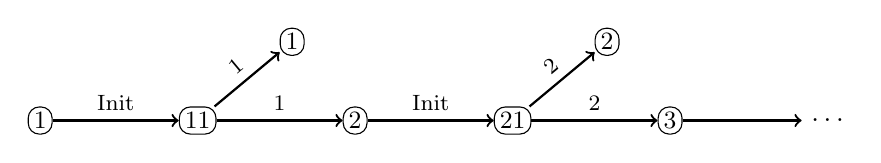
\begin{tikzpicture}
    [hstate/.style={draw,rectangle,rounded corners,inner sep=2pt,font=\small},
     updateLabel/.style={sloped,font=\footnotesize}]
    \def\colSep{2.0}
    \def\rowSep{1}
    \node[hstate] (L1)  at (0,0)                         {$\LL{1}$};
    \node[hstate] (H11) at ($(L1)  + (\colSep,0)$)       {$\HH{1}{1}$};
    \node[hstate] (O1)  at ($(H11) + (.6*\colSep,\rowSep)$) {$\outToken{1}$};
    \node[hstate] (L2)  at ($(H11) + (\colSep,0)$)       {$\LL{2}$};
    \node[hstate] (H21) at ($(L2)  + (\colSep,0)$)       {$\HH{2}{1}$};
    \node[hstate] (O2)  at ($(H21) + (.6*\colSep,\rowSep)$) {$\outToken{2}$};
    \node[hstate] (L3)  at ($(H21) + (\colSep,0)$)       {$\LL{3}$};
    \node[]       (cnt) at ($(L3)  + (\colSep,0)$)       {$\ldots$};
    \path[->,thick]
      (L1)  edge node[above,updateLabel] {Init}          (H11)
      (H11) edge node[above,updateLabel] {\GNNOut{1}}    (O1)
      (H11) edge node[above,updateLabel] {\GNNLabel{1}}  (L2)
      (L2)  edge node[above,updateLabel] {Init}          (H21)
      (H21) edge node[above,updateLabel] {\GNNOut{2}}    (O2)
      (H21) edge node[above,updateLabel] {\GNNLabel{2}}  (L3)
      (L3)  edge                                         (cnt)
    ;
  \end{tikzpicture}
  \end{center}
  \vspace{-2ex}
  \caption{Architecture of \OurMethodShort~models.}
  \vspace{-2ex}
  \label{fig:seq-architecture2}
\end{figure}

We introduce a \emph{node annotation} output model for predicting $\LL{k+1}$
from $\HH{k}{T}$. The prediction is done for each node independently using
a neural network $j(\noderept{\node}{k,T}, \labelsv_\node^{(k)})$ that takes the
concatenation of $\noderept{\node}{k,T}$ and $\labelsv_\node^{(k)}$ as input and outputs a vector of
real-valued scores:
\begin{equation}
    \labelsv_\node^{(k+1)} = \sigma\left(j(\noderept{\node}{k,T},
    \labelsv_\node^{(k)})\right).
\end{equation}

There are two settings for training \OurMethodShorts: specifying
all intermediate annotations $\LL{k}$, or training the full model end-to-end given only
$\LL{1}$, graphs and target sequences.
The former can improve performance when we have domain knowledge about specific
intermediate information that should be represented in the internal state of
nodes, while the latter is more general. We describe both.

\paragraph{Sequence outputs with observed annotations}

Consider the task of making a sequence of predictions for a graph, where each
prediction is only about a part of the graph. In order to
ensure we predict an output for each part of the graph exactly once, it
suffices to have one bit per node, indicating whether the node has been
``explained'' so far.
In some settings, a small number of annotations are sufficient
to capture the state of the output procedure. When this is the case, we
may want to directly input this information into the model via labels
indicating target intermediate annotations. In some cases, these annotations
may be \emph{sufficient}, in that we can define a model where
the \OurMethodMinorShorts~are rendered
conditionally independent given the annotations.

%Suppose we are given a set of disconnected subgraphs as input and our
%goal is to return a set of graph-level classifications---one per subgraph.
%If we wanted to treat this as a sequential output problem, we could
%give the full graph as input and ask for a sequence of classifications
%as output. The prediction tasks at each subgraph are mostly independent,
%but there is a global interaction in that we need to ensure that we
%provide a classification for each subgraph exactly once. This problem
%structure implies that one bit per node, indicating whether the node has
%been ``explained'' so far, suffices to maintain the necessary
%state when outputting the sequence of classifications. After a subgraph
%has been classified, the \emph{explained} bit should be set to 1 for each
%node in the subgraph, and once all nodes have the bit set to 1, it is safe
%to output the \texttt{end} symbol. While the above example is artificially simple, it conveys
%the point that in some settings, a small number of annotations are sufficient
%to capture the state of the output procedure. When this is the case, we
%may want to directly input this information into the model via labels
%indicating target intermediate annotations.

%To do so, we extend the node attribute vector $\labelsv_\node$ to include these
%sequence related annotations $\annotation_\node$.  At each prediction step, we have
%one GNN that produces one output in the output sequence, and another GNN
%that takes the same input and updates $\annotation_\node$ for each
%$\node$, which will be used in the next step. The anntation output
%model is a feedforward neural network that maps the node representations
%$\noderept{\node}{T}$ to the annotations $\annotation_\node$.
%\TODO{this bit is somewhat unclear, as it makes it sound like the output annotations
%are provided as inputs}

In this case, at training time, given the annotations $\LL{k}$ the sequence prediction task
decomposes into single step prediction tasks and can be trained as separate \OurMethodMinorShorts.
At test time, predicted annotations from one step will be used as
input to the next step. This is analogous to training directed graphical models when
data is fully observed.

\paragraph{Sequence outputs with latent annotations}

More generally, when intermediate node annotations $\LL{k}$ are not available during
training, we treat them as hidden units in the network, and train the whole
model jointly by backpropagating through the whole sequence.
%An illustration
%of the \OurMethodShorts~architecture is shown in
%\figref{fig:seq-architecture}.

\comment{
\begin{figure}
    \begin{center}
        \includegraphics[width=0.8\columnwidth]{figs/ggs-nn-architecture.pdf}
    \end{center}
    \caption{Architecture of our \OurMethodShorts~model. The initial node
    attributes $\labelsv_\node^0$ are filled with task related information.  The
    node attribute vectors for intermediate steps can be fully observed,
    partially observed, or fully unobserved (this is the case when we use the
    annotation model to predict the full $\labelsv_\node$).
    \TODO{interesting that we don't need to feed output $t-1$ in at timestep
      $t$. Presumably this is because there is little uncertainty over the
      outputs? E.g., if there were two equally likely outputs, how would we
      know which one we started producing?}
  \TODO{Replace GNN with \OurMethodMinorShort}
    }
    \label{fig:seq-architecture}
\end{figure}
}



%\TODO{(Yujia) how are previous outputs are incorporated as inputs?}
%Case 2: unobserved annotations


%%%%%%%%%%%%%%%%%%%%%%%%%%%%%%%%%%%%%%%%%%%%%%%%%%%%%%%%%%%%%%%%%%%%%%

% \section{Explanatory Examples}

% We discuss and evaluate on illustrative example problems.

\begin{table*}[t!]
\centering
\small
\begin{tabular}{@{}p{0.09\linewidth}|p{0.04\linewidth}|p{0.025\linewidth}p{0.025\linewidth}p{0.025\linewidth}p{0.025\linewidth}p{0.03\linewidth}p{0.025\linewidth}p{0.025\linewidth}p{0.025\linewidth}p{0.03\linewidth}p{0.03\linewidth}p{0.025\linewidth}p{0.03\linewidth}p{0.03\linewidth}p{0.03\linewidth}p{0.03\linewidth}p{0.03\linewidth}}
\hline
category & mean & plane & bag & cap & car & chair & ear-phone & guitar & knife & lamp & laptop & motor-bike & mug & pistol & rocket & skate-board & table \\ \hline
Wu14 \cite{wu2014interactive} & - & 63.20 & - & - & - & 73.47 & - & - & - & 74.42 & - & - & - & - & - & - & 74.76 \\
Yi16 \cite{Yi16} & 81.43 & 80.96 & 78.37 & 77.68 & \textbf{75.67} & 87.64 & 61.89 & 91.79 & 85.36 & 80.59 & 95.58 & \textbf{70.59} & 91.85 & \textbf{85.94} & 53.13 & 69.81 & 75.33 \\
ACNN \cite{boscaini2016learning} & 79.63 & 76.35 & 72.89 & 70.80 & 72.72 & 86.12 & 71.14 & 87.84 & 81.98 & 77.43 & 95.49 & 45.68 & 89.49 & 77.41 & 49.23 & 82.05 & 76.71 \\
Voxel CNN & 79.37 & 75.14 & 72.80 & 73.28 & 70.00 & 87.17 & 63.50 & 88.35 & 79.58 & 74.43 & 93.92 & 58.67 & 91.79 & 76.41 & 51.16 & 65.25 & 77.08   \\ \hline
Ours1 & 83.48 & 80.61 & 81.62 & 76.92 & 73.86 & 88.65 & 74.48 & 89.03 & 85.34 & 83.47 & 95.53 & 62.74 & 92.01 & 80.88 & \textbf{62.10} & 82.23 & 81.36 \\
Ours2 & \textbf{84.74} & \textbf{81.55} & \textbf{81.74} & \textbf{81.94} & 75.16 & \textbf{90.24} & \textbf{74.88} & \textbf{92.97} & \textbf{86.10} & \textbf{84.65} & \textbf{95.61} & 66.66 & \textbf{92.73} & 81.61 & 60.61 & \textbf{82.86} & \textbf{82.13} \\ \hline
\end{tabular}
\caption{IoU for part segmentation on 16 categories. To compute mean IoU, per category IoU is weighted by the corresponding shape number and then averaged. Ours1 represents a variation of our framework without SpecTN and Ours2 corresponds to our full pipeline with SpecTN. On average, our approach outperforms all the baseline including both traditional machine learning and deep learning based methods by a large margin. We also achieves the highest IoU on most of the categories.}
\label{tab:percatseg}
\end{table*}
\label{sec:exp}
Our proposed SyncSpecCNN takes one graph vertex function as input and predicts another as output. As a generic framework, the prediction is not limited to a specific type of graph vertex function and can be tailored towards different goals. To evaluate the effectiveness of our framework, we divide our experiments into five parts. First, we evaluate on a benchmark of 3D shape segmentation~\cite{shapenet2015,Yi16}. Second, we evaluate on keypoint prediction task using a new large scale keypoint annotation dataset. Third, we leverage SyncSpecCNN to learn vertex normal functions and visualize the prediction results qualitatively. Fourth, we perform control experiments to compare different design choices of the framework and analyze the stability of our system under input sampling density variations. Last, we show qualitative results and analyze error patterns.

\subsection{Dataset}
For 3D shape segmentation task, we use a large scale shape part annotation dataset introduced by \cite{Yi16}, which augments a subset of ShapeNet models with semantic part annotations. The dataset contains 16 categories of man-made shapes, with 2 to 6 parts per category. In total there are 16,881 models with expert verified part annotations. In addition, we use the official train/test split provided along with ShapeNet models.

For the keypoint prediction task, we build a new large scale keypoint annotation dataset, containing 1,337 chair models with 10 keypoints per shape, in contrast to traditional small scale dataset \cite{kim2013learning} which has at most 100 shapes annotated per category. These keypoints are all manually annotated by experts with consistency across different shapes. %The goal of this dataset is to allow people evaluating data-driven keypoint prediction algorithms, in contrast to traditional small scale dataset \cite{kim2013learning} which has at most 100 shapes annotated per category.

\subsection{Shape Part Segmentation} 

\myparaly{Per-category shape part segmentation}
We first conduct part segmentation assuming the category label of each shape is known, as the setting in \cite{Yi16}. The task is to predict a part label for each sample point on shapes. We compare our framework with traditional learning-based techniques \cite{wu2014interactive,Yi16} leveraging on local geometric features and shape alignment cues, as well as recent deep learning based approaches \cite{boscaini2016learning} which also fall into the family of spectral CNNs. In addition we design an additional baseline using a 3D volumetric CNN architecture, denoted as Voxel CNN, which generalizes VoxNet~\cite{maturana2015voxnet} for segmentation tasks. The network has 10 convolutional layers without down-sampling and keeps a receptive field of 19 with spatial resolution of 32. We compute per-point features in the preprocessing step as is in \cite{Yi16} and use the same set of input for all baselines except Voxel CNN. The set of input shapes are pre-aligned using a hierarchical joint alignment algorithm described in \cite{shapenet2015}. Point intersection over union (IoU) is used as evaluation metric, averaged across all part classes. Cross-entropy loss is minimized during training. 

We evaluate our framework in two settings, with or without SpecTN, and compare the results in Table~\ref{tab:percatseg}. % In practice, we find that the gain from dilation becomes marginal when SpecTN is used, even though dilation alone helps significantly. While leaving out SpecTN, 
% We used our dilated parametrization with a dilation parameter $\gamma=128$ for convolution.
%We set a dilation parameter $\gamma=128$ for convolution.

Note that on most categories our approach achieves the best performance and on average outperforms state of the art by a large margin. In comparison to \cite{boscaini2016learning},  the state of the art in the family of spectral CNNs, our approach introduces spectral dilated kernel parametrization, which increases the effectiveness of spectral CNN framework.  Moreover, the performance gain from SpecTN shows that synchronizing spectral domains would greatly increase the generalizibility across shapes of different topology and geometry. 

\iffalse
\begin{table*}[t!]
\centering
\small
\begin{tabular}{@{}p{0.04\linewidth}|p{0.05\linewidth}p{0.07\linewidth}|p{0.025\linewidth}p{0.022\linewidth}p{0.022\linewidth}p{0.022\linewidth}p{0.025\linewidth}p{0.025\linewidth}p{0.025\linewidth}p{0.025\linewidth}p{0.025\linewidth}p{0.025\linewidth}p{0.025\linewidth}p{0.025\linewidth}p{0.025\linewidth}p{0.025\linewidth}p{0.025\linewidth}p{0.025\linewidth}}
\hline
& mean partial & mean complete & plane & bag & cap & car & chair & ear-phone & guitar & knife & lamp & laptop & motor-bike & mug & pistol & rocket & skate-board & table \\ \hline
ACNN & 69.21 & 79.63 & 62.73 & 63.26 & 58.90 & 38.25 & 70.59 & \textbf{68.68} & \textbf{88.08} & 74.58 & 61.49 & 87.03 & 31.90 & 79.92 & 62.98 & 35.70 & 68.41 & 76.07 \\ \hline
Ours1 & 76.19 & 83.48 & 71.01 & 77.61 & 64.78 & 56.05 & 78.97 & 68.50 & 84.63 & 82.01 & 73.02 & 91.40 & 40.71 & 87.34 & 72.60 & \textbf{42.53} & 80.61 & 79.55 \\
Ours2 & \textbf{78.02} & \textbf{84.74} & \textbf{74.55} & \textbf{82.58} & \textbf{65.36} & \textbf{58.12} & \textbf{80.41} & 65.55 & 84.75 & \textbf{82.53} & \textbf{77.39} & \textbf{93.15} & \textbf{43.12} & \textbf{90.24} & \textbf{74.71} & 42.17 & \textbf{83.22} & \textbf{80.51} \\ \hline
\end{tabular}
\caption{IoU for part segmentation on incomplete shapes. Note that for comparison, we not only report mean IoU for partial shape part segmentation under "mean partial", but also list mean IoU for complete shape part segmentation under "mean complete". Ours1 represents a variation of our framework without SpecTN and Ours2 corresponds to our full pipeline with SpecTN. On avearge we beat ACNN, the baseline approach, by a large margin and we outperforms ACNN on most shape categories. Moreover, our approach is more robust to data incompleteness since its performance drop is lower in comparison with complete shape segmentation.}
\label{tab:partialseg}
\end{table*}
\fi

\mypara{Cross-category shape part segmentation}
Next we evaluate our approach on the part segmentation task in a cross-category setting. In this task, shape category label is not known during the test phase and for each point the network needs to select one of the part label from all possible part labels in all categories. Cross-category setting introduces larger geometric and topological variance among shapes, thus could help examining the spectral CNN's ability of recognizing objects. At the same time the impact of spectral domain misalignment becomes stronger, providing a better testbed for validating the effectiveness of SpecTN. % Essentially the network needs to have the ability to differentiate shape categories in order to do this task well. 
% Since previous supervised shape segmentation approaches mostly focus on the setting with know shape category labels, 
Since this experiment is proposed to verify design choices of spectral CNN, we mainly compare with \cite{boscaini2016learning}. We mix the 16 categories of shapes in \cite{Yi16} and train a single network for all categories. After predicting point segmentation labels, one can classify shapes through a point-wise majority voting scheme. Point IoU and classification accuracy (Acc) are chosen as the evalution metric for part segmentation and object categorization, respectively. The results are shown in the $2$nd and $3$rd column of Table~\ref{tab:partialseg}.

Our approach outperforms the baseline ACNN by a large margin on both segmentation and classification. Note that ACNN~\cite{boscaini2016learning} does not explicitly conduct multi-scale analysis and is designed for near-isometric 3D shapes with similar spectral domains, thus generalizes less well across a diverse set of shapes. Our framework, in contrast, could effectively capture multi-scale context information, a feature that is highly important for both segmentation and classification. The spectral domain synchronization ability of SpecTN  further improves our generalizability, leading to an extra performance gain as is shown in Table~\ref{tab:partialseg}.

\iffalse
\begin{table}[h!]
\centering
\begin{tabular}{@{}ccc}
\toprule
               & IoU & Classification Acc\\ \midrule
ACNN \cite{boscaini2016learning} & 69.22 & 93.99 \\
Ours without SpecTN  & 79.65 & 99.59 \\
Ours with SpecTN  & \textbf{81.97} & \textbf{99.71} \\ \bottomrule
\end{tabular}
\caption{IoU for cross category part segmentation along with an induced classification accuracy. Even without SpecTN, our approach outperforms the baseline method on both segmentation IoU and classification accuracy, due to its ability of aggregating mult-scale information. Introducing SpecTN further improves the generalizability, resulting in an extra performance gain. }
\label{tab:crosscatseg}
\end{table}
\fi

\mypara{Partial data part segmentation}
To evaluate the robustness of our approach to incomplete data, we conduct part segmentation on simulated scans of 3D shapes from a single viewpoint. To be specific, we generate $N=6$ simulated scans for each 3D shape in the part annotation dataset \cite{Yi16} from random viewpoints, and then use these partial point cloud with part annotations for train and test. All the partial point clouds are normalized to fit into a unit cube. Following the train/test split provided by \cite{shapenet2015}, we train our network to segment shape parts for each category. Again we compare our method with ACNN~\cite{boscaini2016learning}. IoU is used as evaluation metric and the results are shown in the $4$th and $5$th column of Table~\ref{tab:partialseg}.

Our approach outperforms the baseline on partial data part segmentation by a large margin. In particular, from complete shape to partial shape setting, the performance drop of our approach is less significantly than the baseline, reflected by the gap of mean IoU between the complete data setting and the partial setting. It verifies that our method is more robust to data incompleteness. We surmise that the performance of ACNN is heavily influenced by noisy and sensitive principal curvature estimation on partial scans since this step plays a crucial rule in determining its local frames; whereas our approach makes less assumption about quality of the underlying shape.

\begin{table}[t!]
\centering
\small
\begin{tabular}{@{}c|cc|cc}
\hline
& cross cat IoU & Acc & partial & complete\\ \hline
ACNN & 69.22 & 93.99 & 69.21 & 79.63 \\ \hline
Ours1 & 79.65 & 99.59 & 76.19 & 83.48 \\
Ours2 & \textbf{81.97} & \textbf{99.71} & \textbf{78.02} & \textbf{84.74} \\ \hline
\end{tabular}
\caption{The $2$nd and $3$rd column of the table reports IoU for cross category part segmentation along with an induced classification accuracy. $4$th and $5$th column of the table reports IoU for part segmentation on partial shapes and complete shapes correspondingly. Our1 and Our2 corresponds to our framework without and with SpecTN respectively. In all experiments we beat the baseline by a large margin.}
\label{tab:partialseg}
\vspace{-0.6cm}
\end{table}

\iffalse
\todo{
\begin{itemize}
    \item Per-category segmentation
        \subitem Baseline: SigAsia part annotation approach, anisotropic CNN, volumetric cnn
    \item Cross-category segmentation
        \subitem Compare our method with baseline method. show our method has the ability to do simultaneous classification and segmentation among very different graphs.
    \item Partial Data Part Segmentation
        \subitem Quantitatively and qualitatively show how our method performs on partial data. robust to missing points?
\end{itemize}
}
\fi

\subsection{Keypoint Prediction}
Our framework is not limited to part segmentation but could learn more general functions on graphs. In this section, we evaluate our framework on the keypoint prediction task. We associate each keypoint an individual label and assign all the non-keypoints a background class label. The keypoint prediction problem could be treated as a multi-class classification problem and the cross-entropy loss is optimized during training. We evaluate our approach against previous state-of-the-art method \cite{huang2013fine}. \cite{huang2013fine} first jointly aligns all the shapes in 3D space via free-form deformation and then propagates keypoint labels to test shapes from its $K$ nearest training shapes. We manually tune $K$ and report the best performance of this method. Five-folds cross validation is adopted during evaluation, and PCK (percentage of correct keypoints) is used as evaluation metric. We show the PCK curve for the two approaches in Figure~\ref{fig:keypoint}. Each point on a curve indicates fraction of correctly predicted keypoints for a given Euclidean error threshold. Our approach outperforms \cite{huang2013fine}, in particular, more precise predictions can be obtained by our method (see the region close to y-axis).

\iffalse
\todo{
We plan to manually annotate a subset of ShapeNet models and test our algorithm on supervised keypoint prediction tasks. compare with Peter's joint alignment approach.
}
\fi

\subsection{Normal Prediction}
\label{sec:normal}
To further validate the generality of our framework, we leverage our proposed SyncSpecCNN to learn another type of graph vertex function, vertex normal function. Specifically, our SyncSpecCNN takes the XYZ coordinate function of graph vertices as network input and predicts vertex normal as output. The network is trained to minimize the L2 loss between ground truth normals and predicted normals. We use the official train/test split provided by \cite{shapenet2015} and visualize some of the normal prediction results from test set in Figure~\ref{fig:normpred}.

\begin{figure}
 \centering
 \includegraphics[width=1\linewidth]{./fig/visnormal.pdf}
 \caption{We evaluate our framework on normal prediction task. The colors shown on the 3D shape are RGB-coded normals, namely putting XYZ components of normal directions into RGB channels. Our framework could predict reasonable normal directions even on very thin structures.}
 \label{fig:normpred}
\end{figure}

It can be seen our predictions are very close to the ground truth at most of the time.Even on thin structures the normal predictions are still reasonable. One problem of our prediction is that it tends to generate smoothly transiting normals along the boundary while the ground truth is sharper. This is due to the fact that we are using a small number of eigenbases in our experiments, which is not friendly to regression tasks with very high frequency signal as target.

\subsection{Diagnosis}
\myparaly{Spectral Dilated Kernel Parametrization}
 We evaluate our dilated kernel parametrization from two aspects: the basis function choice and kernel scale choice. Table~\ref{tab:kerneldesign} summarizes all the comparison results, as explained below.
 
We explore the expressive power of different kernel basis. In the family of spectral CNN, convolution kernels are parametrized by a linear combination of basis functions, i.e. modulated exponential window in our case. Previous methods have proposed to use different basis functions such as cubic spline basis \cite{bruna2013spectral} and exponential window basis \cite{boscaini2016learning}. Each row of Table~\ref{tab:kerneldesign} corresponds to a basis choice.
 
We also evaluate the effectiveness of multi-scale analysis by changing the spatial sizes of convolution kernels. We compare with two baseline choices: set all kernel size to be the smallest kernel size in the current network; set to be the largest one. Each column of Table~\ref{tab:kerneldesign} corresponds to a kernel scale choice.
 
All numbers are reported on the cross-category part segmentation task, by IoU. We only take the XYZ coordinate function of graph vertices as network input as opposed to handcrafted geometry features which may have already capture some multi-scale information. Also we remove the $7$th and $8$th layers from our network which involves SpecTN and is designed for very large convolution kernels. 

It can be seen that modulated exponential window basis has a better expressive power compared with baselines for our segmentation task. Using multi-scale kernels also enables the aggregation of multi-scale information, thus producing better performance than small or large kernels alone. 
\begin{figure}[t!]
    \centering
    \includegraphics[width=0.8\linewidth]{./fig/kpt_pred_chair.pdf}
    \caption{Keypoint prediction comparison. We draw PCK curves for both methods while changing the error threshold. Our approach outperforms \cite{huang2013fine} on average and has particularly high local accuracy when the error threshold is small, i.e. our approach reaches $pck=0.29$ when error threshold equals $0.01$, while \cite{huang2013fine} reaches $pck=0.16$}
    \label{fig:keypoint}
    \vspace{-0.5cm}
\end{figure}


\begin{table}[h!]
\centering
\small
{
\begin{tabular}{@{}lccc}
\toprule
 & small & large & multiscale \\ \midrule
Cubic Spline & 0.5369 & \multicolumn{1}{c}{-} & \multicolumn{1}{c}{-} \\
Exp Window & 0.6285 & 0.7223 & 0.7386 \\
Modulated Exp Window & 0.6997 & 0.7341 & \textbf{0.7524} \\ \bottomrule
\end{tabular}
}
\caption{We compare different kernel basis and kernel size choices, using cross category part segmentation task for evaluation. IoU is reported in the table. In particular, we compare cubic spline basis \cite{bruna2013spectral}, exponential window basis \cite{boscaini2016learning} and our modulated exponential window. All convolution kernels are parametrized by the same number of parameters and we tweak the hyper parameters of different basis functions so that their spatial sizes are comparable. We also compare three different kernel size choices. "small" indicates using small convolution kernel only; "large" indicates using large convolution kernel only; "multiscale" uses kernels of different sizes in different layers, as in our current design. It's not obvious how to parametrize multi-scale convolution kernels using cubic spline basis functions, therefore we evaluate cubic spline basis with small-sized kernels only.} 
\label{tab:kerneldesign}
\vspace{-0.3cm}
\end{table}

\paragraph{Robustness to Sampling Density Variance}
In this experiment, we evaluate the robustness of our approach w.r.t point cloud density variation. To be specific, we train our SyncSpecCNN for shape segmentation on the point cloud provided by \cite{Yi16} first. Then we downsample the point cloud under different downsample ratio and evaluate our trained model to check how segmentation performance would change. Again we evaluate our approach with/without SpecTN and the result is shown in Figure~\ref{fig:downsample}.
 
By introducing SpecTN, our framework becomes more robust to sampling density variation. Our conjecture is that sampling density variation may result in large spectral space perturbation, therefore being able to synchronize different spectral domains becomes especially important.

\begin{figure}
 \centering
 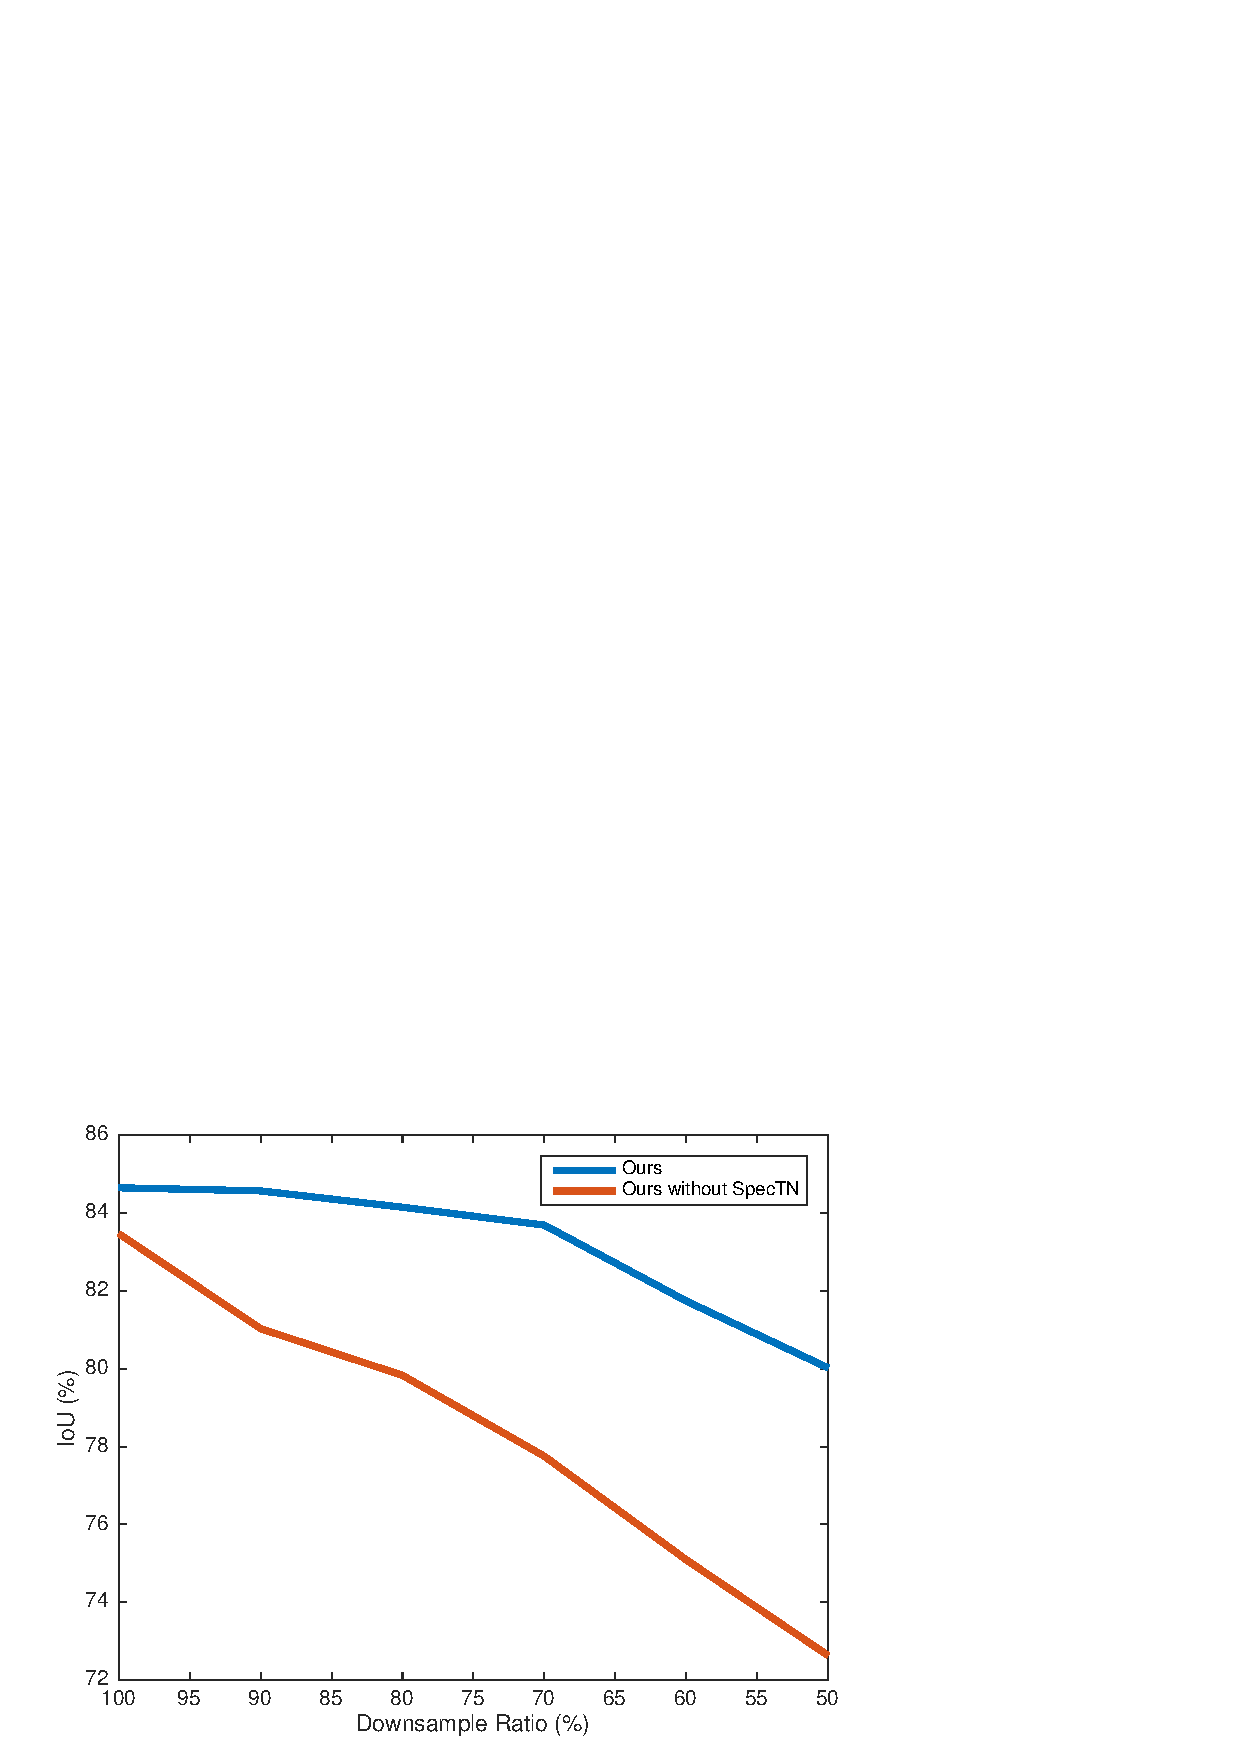
\includegraphics[width=0.8\linewidth]{./fig/downsample.pdf}
 \caption{We evaluate the robustness of our model to sampling density change. Test shapes are downsampled by different ratios and fed into our network. We compute the segmentation IoU for different downsample ratios and show it here. With SpecTN, our framework becomes more robust to sampling density change.}
 \label{fig:downsample}
\end{figure}

%\todo{Visualize joint basis}

\subsection{Qualitative Results and Error Analysis}
Figure~\ref{fig:erroranalysis} shows segmentation results generated from our network on two categories, Chair and Lamp. Representative good results are shown in the first block and  typical error patterns are summarized from the second to fourth blocks.

Most of our segmentation is very close to ground truth as is shown in the first block. We can accurately segment shapes with large geometric or topological variations like wide bench v.s. ordinary chair, pendant lamp v.s. table lamp. The lamp base on the first row and the lampshade on the second row are very similar regarding their local geometry; however, since our network is able to capture large scale context information, it could still differentiate the two and segment shapes correctly.

We observe several typical error patterns in our results. Most segmentation error occurs along part boundaries. %Our network sometimes generates fuzzy part boundaries, especially if the underlying part segments have a very smooth normal transition, as is shown in the second row of the second block. 
There are also cases where the semantic definition of parts has inherent ambiguities. %In these cases, our network may generate predictions slightly different from the ground truth but are still reasonable. 
We also observe a third type of error pattern, in which our prediction might miss a certain part completely, as is shown in the fourth block.

\begin{figure}
    \centering
    \includegraphics[width=\linewidth]{./fig/erroranalysis4.pdf}
    \caption{We visualize some segmentation results from our network prediction. The first block shows typical correct segmentations, notice the huge shape variation we can cover. The second to fourth blocks summarize different error patterns we observe in the results.}
    \label{fig:erroranalysis}
\end{figure}

\iffalse
\todo{
Compare different alternatives of our method
\begin{itemize}
    \item with multiple representatives instead of a single canonical space for spectral synchronization
    \item without join basis learning, visualize joint basis
    \item without dilated kernel, visualize dilated kernel
    \item different kernel choice: polynomial, cubic splines, exponential window, modulated exponential window
    \item different input vertex functions, extrinsic vertex functions help much since it's essentially a combination between extrinsic and intrinsic information for segmentation. intrinsic feature might not help much since the network is intrinsic and captures quite a lot intrinsic information already.
    \item network design, with/without skip link
\end{itemize}
}
\fi

%%%%%%%%%%%%%%%%%%%%%%%%%%%%%%%%%%%%%%%%%%%%%%%%%%%%%%%%%%%%%%%%%%%%%%

\section{Program Verification with \OurMethodShorts}
\label{sect:ProgramVerification}

Our work on \OurMethodShorts{} is motivated by a practical application in
program verification.
A crucial step in automatic program verification is the inference of
\emph{program invariants}, which
%(over-)%
approximate the set of program states
reachable in an execution.
%While a number of techniques for the inference of arithmetic program
%invariants exist, 
Finding invariants about data structures is an open problem.
As an example, consider the simple \texttt{C} function on the right.

\begin{wrapfigure}[7]{r}{6.1cm}
\small\vspace{-2ex}
\begin{alltt}
node* concat(node* a, node* b) \{
  if (a == NULL) return b;
  node* cur = a;
  while (cur.next != NULL)
    cur = cur->next;
  cur->next = b;
  return a; \hfill\}
\end{alltt}
\end{wrapfigure}
To prove that this program indeed concatenates the two lists \texttt{a} and
\texttt{b} and that all pointer dereferences are valid, we need to
(mathematically) characterize the program's heap in each iteration of the loop.
For this, we use \emph{separation logic}~\citep{OHearn01,Reynolds02}, which uses
\emph{inductive predicates} to describe abstract data structures.
For example, a \underline{l}ist \underline{s}egment is defined as $\SLls(x, y)
\equiv x = y \lor \exists v, n . \SLls(n, y) \ast x \mapsto \{\texttt{val}:v,
\texttt{next}:n\}$, where $x \mapsto \{\texttt{val}:v, \texttt{next}:n\}$ means
that $x$ points to a memory region that contains a structure with \texttt{val}
and \texttt{next} fields whose values are in turn $v$ and $n$.
The $\ast$ connective is a conjunction as $\land$ in Boolean logic, but
additionally requires that its operators refer to ``separate'' parts of the
heap.
Thus, $\SLls(\texttt{cur}, \texttt{NULL})$ implies that $\texttt{cur}$ is either
$\texttt{NULL}$, or that it points to two values $v, n$ on the heap, where $n$
is described by $\SLls$ again.
The formula $ \exists t . \SLls(\texttt{a}, \texttt{cur}) \ast
\SLls(\texttt{cur}, \texttt{NULL}) \ast\SLls(\texttt{b}, t)$ is an
\emph{invariant} of the loop (i.e., it holds when entering the loop, and
after every iteration).
Using it, we can prove that no program run will fail due to dereferencing an
unallocated memory address (this property is called \emph{memory safety}) and
that the function indeed concatenates two lists using a Hoare-style verification
scheme~\citep{Hoare69}.

The hardest part of this process is coming up with formulas that describe
data structures, and this is where we propose to use machine
learning.  Given a program, we run it a few times and
extract the state of memory (represented as a graph; see below) at relevant program locations,
and then predict a separation logic formula.
Static program analysis tools (e.g., \citep{Piskac14}) can check whether a
candidate formula is sufficient to prove the desired properties (e.g., memory
safety).

\subsection{Formalization}

\paragraph{Representing Heap State as a Graph}
%
As inputs we consider directed, possibly cyclic graphs representing the heap of
a program. These graphs can be automatically constructed from a program's memory
state.
Each graph node $\heapGNode$ corresponds to an address in memory at which a
sequence of pointers $\heapGNode_0, \ldots, \heapGNode_k$ is stored (we ignore
non-pointer values in this work).
Graph edges reflect these pointer values, i.e., $\heapGNode$ has edges 
labeled with $0, \ldots, k$  that point to nodes $\heapGNode_0, \ldots,
\heapGNode_k$, respectively.
%The node $0$ is special (corresponding to the \texttt{NULL} pointer in programs)
%and may not have outgoing edges.
A subset of nodes are labeled as corresponding to program variables.

An example input graph is displayed as ``Input'' in \figref{fig:annotations2}.
In it, the node id (i.e., memory address) is displayed in the node.
Edge labels correspond to specific fields in the program, e.g., $0$ in our
example corresponds to the \texttt{next} pointer in our example function from
the previous section. For binary trees there are two more types
of pointers \texttt{left} and \texttt{right} pointing to the left and right
children of a tree node.



\paragraph{Output Representation}
%
Our aim is to mathematically describe the shape of the heap.
In our model, we restrict ourselves to a syntactically restricted version of
separation logic, in which formulas are of the form
 $\exists x_1, \ldots, x_n . a_1 \ast \ldots \ast a_m$,
where each atomic formula $a_i$ is either $\SLls(x, y)$ (a list from $x$ to $y$),
$\SLtree(x)$ (a binary tree starting in $x$), or $\SLempty(x)$ (no data
structure at $x$).
%Similar to an arithmetic formula $\phi(x_1, \ldots, x_n)$ which describes
%valuations of variables $x_1, \ldots, x_n$ that satisfy the formula, a
%separation logic formula describes a set of allowed heaps.
%From here on, rather than using names to identify fields of a memory structure, 
%we now use plain sequences of addresses, which are equivalent but
%simpler to model. Thus, $v \mapsto [v_0, \ldots, v_k]$ means that $v$ ``points
%to'' the sequence $[v_0, \ldots, v_k]$ on the heap. 
Existential quantifiers are used to give names to heap nodes which are
needed to describe a shape, but not labeled by a program variable.
For example, to describe a ``panhandle list'' (a list that ends in a
cycle), the first list element on the cycle needs to be named.
In separation logic, this can be expressed as $\exists t . \SLls(x, t)
\ast \SLls(t, t)$.

\paragraph{Data}
We can generate synthetic (labeled) datasets for this problem.
For this, we fix a set of predicates such as $\SLls$ and $\SLtree$ (extensions
could consider doubly-linked list segments, multi-trees, $\ldots$) together with
their inductive definitions.
%We also decide on a set of shapes constructed from these
%basic predicates, e.g. simple lists, cyclic lists, panhandle lists,
%\ldots.
Then we enumerate separation logic
formulas instantiating our predicates using a given set of program variables.
Finally,
for each formula, we enumerate heap graphs satisfying that
formula. The result is a dataset consisting of pairs of heap graphs and
associated formulas that are used by our learning
procedures.


\subsection{Formulation as \OurMethodShorts}

It is easy to obtain
the node annotations for the intermediate prediction steps from the data
generation process. So we train a variant of
\OurMethodShort~with observed annotations (observed at training time; not test time)
to infer formulas from heap graphs.
Note that it is also possible to use an unobserved
\OurMethodShort~variant and do end-to-end learning. The procedure breaks down
the production of a separation logic formula into a sequence of
steps. We first decide whether to declare existential variables, and if so,
choose which node corresponds to the variable.
Once we have declared existentials, we iterate over all variable names
and produce a separation logic formula describing the data
structure rooted at the node corresponding to the current variable.

The full algorithm for predicting separation logic formula appears below, as
\algoref{alg:seplogic-prediction}.
We use three explicit node annotations, namely \emph{is-named} (heap node labeled by
program variable or declared existentially quantified variable), \emph{active} (cf. algorithm) and \emph{is-explained} (heap node is
part of data structure already predicted).
Initial node labels can be directly computed from the input graph: ``is-named''
is on for nodes labeled by program variables, ``active'' and ``is-explained''
are always off (done in line 2).
The commented lines in the algorithm are implemented using a
\OurMethodMinorShort, i.e., \algoref{alg:seplogic-prediction} is an instance of
our \OurMethodShort{} model.
An illustration of the beginning of a run of the algorithm is shown in
\figref{fig:annotations2}, where each step is related to one line of the
algorithm.



\begin{figure}
  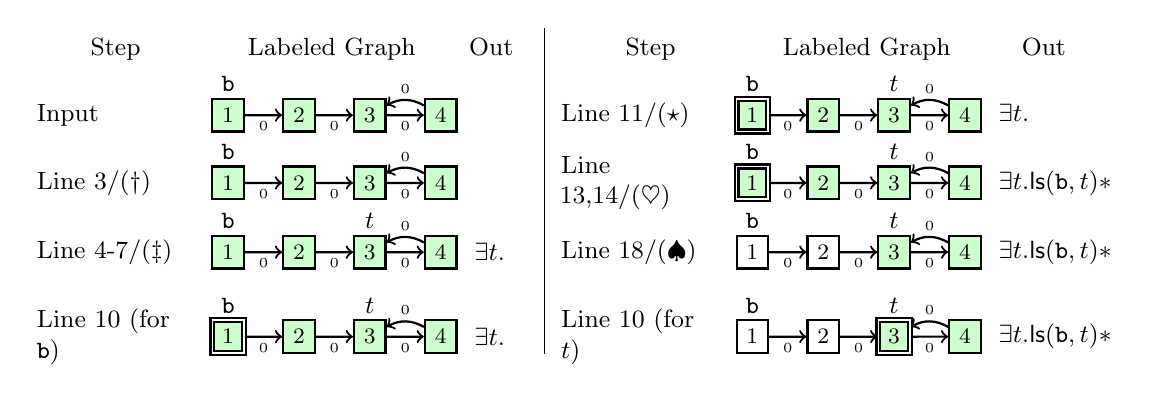
\begin{tikzpicture}[heapgraph,scale=.9]
  \def\rowSep{.35}
  \def\colSep{.1}
  \def\nodeStep{1}
  \node[colLabel] (labelStep)  at (0,0)                        {Step};
  \node[colLabel] (labelGraph) at ($(labelStep) + (3.05,0)$)   {Labeled Graph};
  \node[colLabel] (labelOut)   at ($(labelGraph) + (2.35,0)$)  {Out\phantom{p}};

  \node[stepLabel,anchor=north]               (0labelStep) at ($(labelStep.south) + (0, -\rowSep)$) {Input};
  \node[anchor=west,list,label=90:\texttt{b}] (0b)         at ($(0labelStep.east) + (\colSep,0)$)   {$1$};
  \node[list]                                 (0bn)        at ($(0b)              + (\nodeStep,0)$) {$2$};
  \node[list]                                 (0t)         at ($(0bn)             + (\nodeStep,0)$) {$3$};
  \node[list]                                 (0tn)        at ($(0t)              + (\nodeStep,0)$) {$4$};
  \node[anchor=west,outLabel]                 (0labelOut)  at ($(0tn.east)        + (\colSep,0)$)   {};
  \path[->, thick]
    (0b)  edge node[below,heapEdgeLabel] {$0$} (0bn)
    (0bn) edge node[below,heapEdgeLabel] {$0$} (0t)
    (0t)  edge node[below,heapEdgeLabel] {$0$} (0tn)
    (0tn) edge[bend right] node[above,heapEdgeLabel] {$0$} (0t)
  ;

  \node[stepLabel,anchor=north]               (1labelStep) at ($(0labelStep.south)+ (0, -\rowSep)$) {Line 3/$(\dagger)$};
  \node[anchor=west,list,label=90:\texttt{b}] (1b)         at ($(1labelStep.east) + (\colSep,0)$)   {$1$};
  \node[list]                                 (1bn)        at ($(1b)              + (\nodeStep,0)$) {$2$};
  \node[list,label=90:$\phantom{t}$]          (1t)         at ($(1bn)             + (\nodeStep,0)$) {$3$};
  \node[list]                                 (1tn)        at ($(1t)              + (\nodeStep,0)$) {$4$};
  \node[anchor=west,outLabel]                 (1labelOut)  at ($(1tn.east)        + (\colSep,0)$)   {};
  \path[->, thick]
    (1b)  edge node[below,heapEdgeLabel] {$0$} (1bn)
    (1bn) edge node[below,heapEdgeLabel] {$0$} (1t)
    (1t)  edge node[below,heapEdgeLabel] {$0$} (1tn)
    (1tn) edge[bend right] node[above,heapEdgeLabel] {$0$} (1t)
  ;

  \node[stepLabel,anchor=north]               (2labelStep) at ($(1labelStep.south)+ (0, -\rowSep)$) {Line 4-7/$(\ddagger)$};
  \node[anchor=west,list,label=90:\texttt{b}] (2b)         at ($(2labelStep.east) + (\colSep,0)$)   {$1$};
  \node[list]                                 (2bn)        at ($(2b)              + (\nodeStep,0)$) {$2$};
  \node[list,label=90:$t$]                    (2t)         at ($(2bn)             + (\nodeStep,0)$) {$3$};
  \node[list]                                 (2tn)        at ($(2t)              + (\nodeStep,0)$) {$4$};
  \node[anchor=west,outLabel]                 (2labelOut)  at ($(2tn.east)        + (\colSep,0)$)   {$\exists t .$};
  \path[->, thick]
    (2b)  edge node[below,heapEdgeLabel] {$0$} (2bn)
    (2bn) edge node[below,heapEdgeLabel] {$0$} (2t)
    (2t)  edge node[below,heapEdgeLabel] {$0$} (2tn)
    (2tn) edge[bend right] node[above,heapEdgeLabel] {$0$} (2t)
  ;

  \node[stepLabel,anchor=north]               (3labelStep) at ($(2labelStep.south)+ (0, -\rowSep)$) {Line 10 (for \texttt{b})};
  \node[anchor=west,list,active,label=90:\texttt{b}] (3b)  at ($(3labelStep.east) + (\colSep,0)$)   {$1$};
  \node[list]                                 (3bn)        at ($(3b)              + (\nodeStep,0)$) {$2$};
  \node[list,label=90:$t$]                    (3t)         at ($(3bn)             + (\nodeStep,0)$) {$3$};
  \node[list]                                 (3tn)        at ($(3t)              + (\nodeStep,0)$) {$4$};
  \node[anchor=west,outLabel]                 (3labelOut)  at ($(3tn.east)        + (\colSep,0)$)   {$\exists t .$};
  \path[->, thick]
    (3b)  edge node[below,heapEdgeLabel] {$0$} (3bn)
    (3bn) edge node[below,heapEdgeLabel] {$0$} (3t)
    (3t)  edge node[below,heapEdgeLabel] {$0$} (3tn)
    (3tn) edge[bend right] node[above,heapEdgeLabel] {$0$} (3t)
  ;

  \draw[-] ($(labelOut.north east) + (.1, 0)$) -- ($(labelOut.north east) + (.1, -4.6)$);
  \node[colLabel] (labelStep')  at ($(labelOut.east) + (1.6,0)$) {Step};
  \node[colLabel] (labelGraph') at ($(labelStep') + (3.05,0)$)   {Labeled Graph};
  \node[colLabel] (labelOut')   at ($(labelGraph') + (2.6,0)$)  {Out\phantom{p}};

  \node[stepLabel,anchor=west]                (4labelStep) at ($(0labelStep.east) + (4.9, 0)$)      {Line 11/$(\star)$};
  \node[anchor=west,list,active,label=90:\texttt{b}] (4b)  at ($(4labelStep.east) + (\colSep,0)$)   {$1$};
  \node[list]                                 (4bn)        at ($(4b)              + (\nodeStep,0)$) {$2$};
  \node[list,label=90:$t$]                    (4t)         at ($(4bn)             + (\nodeStep,0)$) {$3$};
  \node[list]                                 (4tn)        at ($(4t)              + (\nodeStep,0)$) {$4$};
  \node[anchor=west,outLabel]                 (4labelOut)  at ($(4tn.east)        + (\colSep,0)$)   {$\exists t . \phantom{\SLls(\texttt{b},t)}$};
  \path[->, thick]
    (4b)  edge node[below,heapEdgeLabel] {$0$} (4bn)
    (4bn) edge node[below,heapEdgeLabel] {$0$} (4t)
    (4t)  edge node[below,heapEdgeLabel] {$0$} (4tn)
    (4tn) edge[bend right] node[above,heapEdgeLabel] {$0$} (4t)
  ;

  \node[stepLabel,anchor=west]                (5labelStep) at ($(1labelStep.east) + (4.9, 0)$)      {Line 13,14/$(\heartsuit)$};
  \node[anchor=west,list,active,label=90:\texttt{b}] (5b)  at ($(5labelStep.east) + (\colSep,0)$)   {$1$};
  \node[list]                                 (5bn)        at ($(5b)              + (\nodeStep,0)$) {$2$};
  \node[list,label=90:$t$]                    (5t)         at ($(5bn)             + (\nodeStep,0)$) {$3$};
  \node[list]                                 (5tn)        at ($(5t)              + (\nodeStep,0)$) {$4$};
  \node[anchor=west,align=left,outLabel]      (5labelOut)  at ($(5tn.east)        + (\colSep,0)$)   {$\exists t . \SLls(\texttt{b},t) \ast$};
  \path[->, thick]
    (5b)  edge node[below,heapEdgeLabel] {$0$} (5bn)
    (5bn) edge node[below,heapEdgeLabel] {$0$} (5t)
    (5t)  edge node[below,heapEdgeLabel] {$0$} (5tn)
    (5tn) edge[bend right] node[above,heapEdgeLabel] {$0$} (5t)
  ;

  \node[stepLabel,anchor=west]                (6labelStep) at ($(2labelStep.east) + (4.9, 0)$)      {Line 18/$(\spadesuit)$};
  \node[anchor=west,list,explained,label=90:\texttt{b}] (6b) at ($(6labelStep.east)+(\colSep,0)$)   {$1$};
  \node[list,explained]                       (6bn)        at ($(6b)              + (\nodeStep,0)$) {$2$};
  \node[list,label=90:$t$]                    (6t)         at ($(6bn)             + (\nodeStep,0)$) {$3$};
  \node[list]                                 (6tn)        at ($(6t)              + (\nodeStep,0)$) {$4$};
  \node[anchor=west,align=left,outLabel]      (6labelOut)  at ($(6tn.east)        + (\colSep,0)$)   {$\exists t . \SLls(\texttt{b},t) \ast$};
  \path[->, thick]
    (6b)  edge node[below,heapEdgeLabel] {$0$} (6bn)
    (6bn) edge node[below,heapEdgeLabel] {$0$} (6t)
    (6t)  edge node[below,heapEdgeLabel] {$0$} (6tn)
    (6tn) edge[bend right] node[above,heapEdgeLabel] {$0$} (6t)
  ;

  \node[stepLabel,anchor=west]                (7labelStep) at ($(3labelStep.east) + (4.9, 0)$)      {Line 10 (for $t$)};
  \node[anchor=west,list,explained,label=90:\texttt{b}] (7b) at ($(7labelStep.east)+(\colSep,0)$)   {$1$};
  \node[list,explained]                       (7bn)        at ($(7b)              + (\nodeStep,0)$) {$2$};
  \node[list,active,label=90:$t$]             (7t)         at ($(7bn)             + (\nodeStep,0)$) {$3$};
  \node[list]                                 (7tn)        at ($(7t)              + (\nodeStep,0)$) {$4$};
  \node[anchor=west,align=left,outLabel]      (7labelOut)  at ($(7tn.east)        + (\colSep,0)$)   {$\exists t . \SLls(\texttt{b},t) \ast$};
  \path[->, thick]
    (7b)  edge node[below,heapEdgeLabel] {$0$} (7bn)
    (7bn) edge node[below,heapEdgeLabel] {$0$} (7t)
    (7t)  edge node[below,heapEdgeLabel] {$0$} (7tn)
    (7tn) edge[bend right] node[above,heapEdgeLabel] {$0$} (7t)
  ;
\end{tikzpicture}
%%% Local Variables:
%%% mode: latex
%%% TeX-master: "main"
%%% End:

 \vspace{-4ex}
 \caption{Illustration of the first 8 steps to predict a separation logic formula from
   a memory state. Label \emph{is-named} signified by variable near node,
   \emph{active} by double border, \emph{is-explained} by white fill.}
 \label{fig:annotations2}
\end{figure}

\begin{algorithm}
  \begin{algorithmic}[1]
    \Require Heap graph $\graph$ with named program variables
    \State{$\LLSym{} \leftarrow $ compute initial labels from $\graph$}
    \State{$\HHSym{} \leftarrow $ initialize node vectors by $0$-extending
      $\LLSym{}$}
    \While{$\exists$ quantifier needed}\Comment{\textbf{Graph-level Classification ($\dagger$)}}
      \State{$t \leftarrow$ fresh variable name}
      \State{$v \leftarrow$ pick node}
        \Comment{\textbf{Node Selection ($\ddagger$)}}      
      \State{$\LLSym{} \leftarrow$ turn on ``is-named'' for $v$ in $\LLSym{}$}
      \State{\algoutput{} ``$\exists t . $''}
    \EndWhile
    \For{node $v_\ell$ with label ``is-named'' in $\LLSym{}$}
      \State{$\HHSym{} \leftarrow$ initialize node vectors, turn on ``active'' label for $v_\ell$ in $\LLSym{}$}
      \State{$\mathit{pred} \leftarrow$ pick data structure predicate}
        \Comment{\textbf{Graph-level Classification ($\star$)}}
      \If{$\mathit{pred} = \SLls$}
        \State{$\ell_{\mathit{end}} \leftarrow$ pick list end node}
          \Comment{\textbf{Node Selection ($\heartsuit$)}}
        \State{\algoutput{} ``$\SLls(\ell, \ell_{\mathit{end}})~\ast$''}
      \Else{}
        \State{\algoutput{} ``$\mathit{pred}(\ell)~\ast$''}
      \EndIf
      \State{$\LLSym{} \leftarrow$ update node annotations in $\LLSym{}$}
        \Comment{\textbf{Node Annotation ($\spadesuit$)}}
    \EndFor
  \end{algorithmic}
  \caption{Separation logic formula prediction procedure}
  \label{alg:seplogic-prediction}
\end{algorithm}

%\TODO{is there anything to say about the no-annotation version?}


\subsection{Model Setup Details}
We use the full \OurMethodShort~model
where $\GNNOut{k}$ and $\GNNLabel{k}$ have separate propagation models.
For all the \OurMethodMinorShort~components in the \OurMethodShort~pipeline,
we unrolled the propagation process for 10 time steps. The
\OurMethodShorts~associated with step ($\dagger$) (deciding wheter
more existentially quantified variable need to be declared) and ($\ddagger$)
(identify which node need to be declared as existentially quantified) uses
$D=16$ dimensional node representations.  For all other
\OurMethodShort~components, $D=8$ is used.  Adam \citep{kingma2014adam} is
used for optimization, the models are trained on minibatches of 20 graphs, and
optimized until training error is very low. For the graph-level classification tasks, we also
artificially balanced classes to have even number of examples from each class
in each minibatch. All the \OurMethodShort~components contain less than 5k
parameters and no overfitting is observed during training.


\subsection{Batch Prediction Details}
\label{appendix:batch-prediction}

In practice, a set of heap graphs will be given as input and a single output
formula is expected to describe and be consistent with all the input graphs.
The different heap graphs can be snapshots of the heap state at different
points in the program execution process, or different runs of the same program
with different inputs. We call this the ``batch prediction'' setup contrasting
with the single graph prediction described in the main paper.

To make batch predictions, we run one \OurMethodShort~for each graph
simultaneously. For each prediction step, the outputs of all the \OurMethodShorts~at
that step across the batch of graphs are aggregated.

For node selection outputs, the common named
variables link nodes on different graphs togeter, which is the key for
aggregating predictions in a batch.  We compute the score for a particular named
variable $t$ as $o_t = \sum_g o^g_{\nodes_g(t)}$, where $\nodes_g(t)$ maps
variable name $t$ to a node in graph $g$, and $o^g_{\nodes_g(t)}$ is the output score for named
variable $t$ in graph $g$. When applying a softmax over all names using $o_t$
as scores, this is equivalent to a model that computes $p(toselect =
t)=\prod_g p_g(toselect=\nodes_g(t))$.

For graph-level classification outputs, we add up scores of a particular class
across the batch of graphs, or equivalently compute $p(class=k)=\prod_g
p_g(class=k)$.
Node annotation outputs are updated for each graph independently as different
graphs have completely different set of nodes.  However, when the algorithm tries to
update the annotation for one named variable, the nodes
associated with that variable in all graphs are updated.
During training, all labels for intermediate steps are available to us from the data
generation process, so the training process again can be decomposed to single
output single graph training.

%It is possible to train \OurMethodMinorShorts~end-to-end in this batch prediction setup,
%we leave this to the future work.

A more complex scenario allowing for nested data structures (e.g., list of lists) was discussed in
\cite{brockschmidt2015learning}.
We have also successfully extended the \OurMethodShort~model to this case.
More details on this can be found in Appendix
\ref{appendix:nested-prediction}.


\subsection{Experiments. }
\label{sec:program-verification-results}

For this paper, we produced a dataset of 327 formulas that involves three
program variables, with 498 graphs per formula, yielding around 160,000
formula/heap graph combinations.
To evaluate, we split the data into training, validation and test
sets using a 6:2:2 split on the formulas (i.e., the formulas in the test set
were not in the training set). We measure correctness by
whether the formula predicted at test time is logically equivalent to the
ground truth; equivalence is approximated by canonicalizing names and order
of the formulas and then comparing for exact equality.

We compared our \OurMethodShort-based model with a method we developed
earlier~\citep{brockschmidt2015learning}.
The earlier approach treats each prediction step as standard classification,
and requires complex, manual, problem-specific feature
engineering, to achieve
an accuracy of 89.11\%.
In contrast, our new model was trained with no feature engineering and very
little domain knowledge and achieved an accuracy of 89.96\%.

An example heap graph and the corresponding separation logic formula found by
our \OurMethodShort~model is shown in
\figref{fig:appendix-heap-graph-example}. This example also involves nested
data structures and the batching extension developed in the previous section.

\begin{figure}
    \begin{center}
        \includegraphics[width=0.5\textwidth]{figs/appendix-heap-graph-example.png}
    \end{center}
    \caption{A heap graph example that contains two named variables
        \texttt{arg1} and \texttt{arg2}, and one isolated \SLnull~node (node 1). All the
    edges to \SLnull~are not shown here for clarity. The numbers on edges
    indicate different edge types.  Our \OurMethodShort~model successfully
    finds the right
formula $\SLls(\texttt{arg1}, \SLnull, \lambda t_1 \rightarrow \SLls(t_1,
\SLnull, \SLNone)) * \SLtree(\texttt{arg2}, \lambda t_2 \rightarrow \exists
e_1. \SLls(t_2, e_1, \SLNone) * \SLls(e_1, e_1, \SLNone))$.}
    \label{fig:appendix-heap-graph-example}
\end{figure}


We have also successfully used our new model in a program verification
framework, supplying needed program invariants to a theorem prover to prove
correctness of a collection of list-manipulating algorithms such as insertion
sort.
The following Table \ref{table:seplogic-list-invariants} lists a set of benchmark list manipulation programs and
the separation logic formula invariants found by the \OurMethodShort~model,
which were successfully used in a verification framework to prove the
correctness of corresponding programs. A further extension of the current
pipeline has been shown to be able to successfully prove more sophisticated
programs like sorting programs and various other list-manipulating programs.

\begin{table}
\begin{center}
\begin{tabular}{ll}
\toprule
Program & Invariant Found \\
\midrule
Traverse1 & $\SLls(\SLlst,\SLcurr) * \SLls(\SLcurr,\SLnull)$ \\
Traverse2 & $ \SLcurr \ne \SLnull *
\SLlst \ne \SLnull * \SLls(\SLlst,\SLcurr) * \SLls(\SLcurr,\SLnull)$ \\
Concat & $\texttt{a} \ne \SLnull * a \ne b * b \ne \SLcurr * \SLcurr\ne
\SLnull$ \\
& $* \SLls(\SLcurr, \SLnull) * \SLls(a, \SLcurr) * \SLls(b, \SLnull)$ \\
Copy & $\SLls(\SLcurr, \SLnull) * \SLls(\SLlst, \SLcurr) * \SLls(\texttt{cp},
\SLnull) $ \\
Dispose & $\SLls(\SLlst, \SLnull)$ \\
Insert & $\SLcurr\ne\SLnull * \SLcurr\ne \SLelt * \SLelt\ne \SLnull * \SLelt\ne
\SLlst* \SLlst\ne \SLnull$ \\
& $* \SLls(\SLelt, \SLnull) * \SLls(\SLlst, \SLcurr) * \SLls(\SLcurr, \SLnull)$ \\
Remove & $\SLcurr\ne \SLnull * \SLlst\ne \SLnull * \SLls(\SLlst, \SLcurr) *
\SLls(\SLcurr, \SLnull)$ \\
\bottomrule
\end{tabular}
\caption{Example list manipulation programs and the separation logic formula
invariants the \OurMethodShort~model founds from a set of input graphs. The
``$\ne$'' parts are produced by
a deterministic procedure that goes through all the named program variables in
all graphs and checks for inequality.}
\label{table:seplogic-list-invariants}
\end{center}
\end{table}


%%%%%%%%%%%%%%%%%%%%%%%%%%%%%%%%%%%%%%%%%%%%%%%%%%%%%%%%%%%%%%%%%%%%%%

\section{Related Work}

The most closely related work is GNNs, which we have discussed at
length above.
\cite{micheli2009neural} proposed another
closely related model that differs from GNNs mainly in the output model.
GNNs have been applied in several domains
\citep{gori2005new,di2006comparison,scarselli2009graph,uwents2011neural}, but they
do not appear to be in widespread use in the ICLR community.
Part of our aim here is to publicize GNNs as a useful and interesting
neural network variant. 
%\cite{micheli2009neural} uses similar convolutional like updates on a graph structure,
%training the model by adding a single hidden unit at a time, then freezing
%weights for all but the most recently added unit.

An analogy can be drawn between 
our adaptation from GNNs to \OurMethodMinorShorts, to the work of
\cite{domke2011parameter} and \cite{stoyanov2011empirical} in the structured prediction setting.
There belief propagation (which must be run to near convergence to
get good gradients) is replaced with truncated belief propagation updates, and
then the model is trained so that the truncated iteration produce good
results after a fixed number of iterations.
Similarly, Recursive Neural Networks
\citep{goller1996learning,socher2011parsing} being extended to Tree LSTMs
\citep{tai2015improved} is analogous to our using of GRU updates in
\OurMethodMinorShorts~instead of the standard GNN recurrence with the aim of
improving the long-term propagation of information across a graph structure.

The general idea expressed in this paper of assembling
problem-specific neural networks as a composition of learned
components has a long history, dating back at least to the work of
\cite{hinton1988representing} on assembling neural networks according
to a family tree structure in order to predict relations between
people. Similar ideas appear in \cite{hammer2004neural} and \cite{bottou2014machine}.

Graph kernels
\citep{shervashidze2011weisfeiler,kashima2003marginalized} can be used
for a variety of kernel-based learning tasks with graph-structured
inputs, but we are not aware of work that learns the kernels and
outputs sequences.  \cite{perozzi2014deepwalk} convert graphs into sequences by
following random walks on the graph then learns node embeddings using
sequence-based methods.
%Graph transformer networks \citep{bottou1997global,lecun1998gradient}
%are a general framework for mapping from graphs to graphs via a series
%of differentiable operations, but we are unaware of them being used in
%a similar manner as GNNs (e.g., iteratively propagating vector
%representations of nodes around a graph).
\cite{sperduti1997supervised} map graphs to graph vectors then
classify using an output neural network.
There are several models that make use of similar propagation of node
representations on a graph structure.
\cite{bruna2013spectral} generalize
convolutions to graph structures.  The difference between their work
and GNNs is analogous to the difference between convolutional and
recurrent networks.
\cite{duvenaud2015convolutional} also consider convolutional like
operations on graphs, building a learnable, differentiable variant of
a successful graph feature.
%%%% This one is too tailored for
%relational databases - the `graph' structure is not the main thing; and
%relations do not need to be represented as graphs.
%
%Relational neural networks
%\citep{uwents2005classifying} are tailored to a
%relational database structure; the propagation unrolls
%iteration of cyclic graphs a fixed number of steps to get a similar
%unrolling to what we use.
\cite{lusci2013deep} converts an arbitrary
undirected graph to a number of different DAGs with different
orientations and then propagates node representations inwards towards
each root, training an ensemble of models.
In all of the above, the focus is on one-step problems.

GNNs and our extensions have many of the same desirable properties of
pointer networks \citep{vinyals2015pointer};  when using
node selection output layers, nodes from the input can be chosen as outputs.
There are two main differences:~first,
in GNNs the graph structure is explicit, which makes the models less general
but may provide stronger generalization ability; 
second, pointer networks require that each node has
properties (e.g., a location in space), while GNNs can represent
nodes that are defined only by their position in the graph, which 
makes them more general along a different dimension.

\OurMethodShorts~are related to soft alignment and attentional models
(e.g., \cite{bahdanau2014neural,kumar2015ask,sukhbaatar2015end}) in two respects:~first, the graph
representation in \eqref{eq:graph-representation} uses context to
focus attention on which nodes are important to the current decision;
second, node annotations in the program verification example keep
track of which nodes have been explained so far, which gives an
explicit mechanism for making sure that each node in the input
has been used over the sequence of producing an output.


%%%%%%%%%%%%%%%%%%%%%%%%%%%%%%%%%%%%%%%%%%%%%%%%%%%%%%%%%%%%%%%%%%%%%%

\section{Discussion}
\label{sec:discussion}

\paragraph{What is being learned?}

\begin{wrapfigure}[4]{r}{3cm}
\small\vspace{-4ex}
\begin{alltt}
 B is E
 E has_fear H
 eval B has_fear
\end{alltt}
\end{wrapfigure}
It is instructive to consider what is being learned by the
\OurMethodMinorShorts. To do so, we can draw analogy between how the bAbI task 15
would be solved via
a logical formulation. As an example, consider the subset of lines
needed to answer one example on the right.

%\begin{verbatim}
%B is E
%E has_fear H
%eval B has_fear
%\end{verbatim}
 
To do logical reasoning, we would need not only a logical encoding of
the facts present in the story but also the background world knowledge encoded as
inference rules such as 
\begin{align}
\texttt{is(x, y)} \wedge \texttt{has-fear(y, z)} \implies \texttt{has-fear(x, z)}.
\end{align}
Our encoding of the tasks simplifies the parsing of the story into
graph form, but it does not provide any of the background knowledge. 
The \OurMethodMinorShort~model can be seen as learning this,
with results stored in the neural network weights. 

\comment{
To do logical reasoning, we would need not only a logical encoding of
the facts present in the story but also the background world knowledge encoded as
inference rules such as 
\begin{align}
\texttt{is(x, y)} \wedge \texttt{has-fear(y, z)} \implies \texttt{has-fear(x, z)}.
\end{align}
Our encoding of the tasks simplifies the parsing of the story into
graph form, but it does not provide any of the background world knowledge.
Thus, the \OurMethodMinorShort~model can be seen as learning the background world knowledge,
with results stored in the neural network weights.
}

\paragraph{Discussion}

The results in the paper show that \OurMethodShorts~have
desirable inductive biases across a range of problems that
have some intrinsic graph structure to them, and we believe
there to be many more cases where \OurMethodShorts~will be
useful. There are, however, some limitations that need to be overcome to
make them apply even more broadly. Two limitations that we mentioned
previously are that the bAbI task translation does not incorporate
temporal order of inputs or ternary and higher order relations.
We can imagine several possibilities for lifting these restrictions, such
as concatenating a series of \OurMethodMinorShorts, where there is one
\OurMethodMinorShorts~for each edge, and representing
higher order relations as factor graphs. 
A more significant challenge is how to handle less structured input
representations. For example, in the bAbI tasks it would be desirable
not to use the symbolic form of the inputs. One possible approach
is to incorporate less structured inputs, and latent vectors, in our 
\OurMethodShorts.
However, experimentation is
needed to find the best way of addressing these issues.

%Mapping from free-form
%sentences to more symbolic representations is a commonly studied
%but hard problem in natural language processing
%\cite{gildea2002automatic,banarescu2012abstract}

The current \OurMethodShorts~formulation specifies a question only after
all the facts have been consumed. This implies that the network must try
to derive all consequences of the seen facts and store all pertinent information
to a node within its node representation. This is likely not ideal;
it would be preferable to develop methods that take the question as an initial
input, and then dynamically derive the facts needed to answer the question.

We are optimistic about the further applications of \OurMethodShorts.
We are particularly interested in continuing to develop end-to-end learnable
systems that can learn about semantic properties of programs, that can
learn more complicated graph algorithms,  and in
applying these ideas to problems that
require reasoning over knowledge bases and databases.
More generally, we consider these graph neural networks as representing a
step towards a model that can combine structured representations with the
powerful algorithms of deep learning, with the aim of taking advantage of known
structure while learning and inferring how to reason with and extend 
these representations.
% Perhaps it would be possible
%to combine \OurMethodShorts~with a model that can handle less structured
%inputs and get the best of both worlds.

\section*{Acknowledgements}
We thank Siddharth Krishna, Alex Gaunt,
Emine Yilmaz, Milad Shokouhi,
and Pushmeet Kohli for useful
conversations and Douwe Kiela for comments on an earlier draft of the
paper.

\bibliography{refs}
\bibliographystyle{iclr2016_conference}

\section{Positive Definiteness of~$K$}\label{sec:appendixA}
To show that the kernel~$K$ defined in~(\ref{eq:kernel}) is positive definite
(p.d.), we simply use elementary rules from the kernel literature described in
Sections 2.3.2 and 3.4.1 of~\cite{shawe2004}.  A linear combination of p.d. kernels with non-negative weights is also p.d. (see Proposition 3.22
of\cite{shawe2004}), and thus it is sufficient to show that for all $\z,\z'$
in~$\Omega$, the following kernel on $\Omega \to \HH$ is p.d.:
\begin{displaymath}
   (\varphi,\varphi') \mapsto \big\|\varphi(\z)\big\|_\HH  \normH{\varphi'(\z')} e^{-\frac{1}{2\sigma^2} \normH{\tildephi(\z)-\tildephi'(\z')}^2}.
\end{displaymath}
Specifically, it is also sufficient to
show that the following kernel on $\HH$ is p.d.:
\begin{displaymath}
   (\phi,\phi') \mapsto \big\|{\phi}\big\|_\HH  \normH{\phi'} e^{-\frac{1}{2\sigma^2} \normH{\frac{\phi}{\|\phi\|_\HH}-\frac{\phi'}{\|\phi'\|_\HH}}^2}.
\end{displaymath}
with the convention $\phi/\|\phi\|_\HH=0$ if~$\phi=0$.
This is a pointwise product of two kernels and is p.d. when each of the two
kernels is p.d. The first one is obviously p.d.: $(\phi,\phi') \mapsto
\|{\phi}\|_\HH  \normH{\phi'}$. The second one is a composition of the Gaussian
kernel---which is p.d.---, with feature maps $\phi/\|\phi\|_\HH$ of a
normalized linear kernel in~$\HH$.  This composition is p.d. according to
Proposition 3.22, item (v) of~\cite{shawe2004} since the normalization does
not remove the positive-definiteness property.

\section{List of Architectures Reported in the Experiments}\label{appendix:arch}
We present in details the architectures used in the paper in Table~\ref{table:arch}.
\begin{table}[hbtp]
   \centering
   \begin{tabular}{|*{9}{c|}}
      \hline
      Arch. & $N$ & $m_1$  & $p_1$  &  $\gamma_1$ & $m_2$ &  $p_2$ & $S$  &  $\sharp$ param\\
      \hline
      \hline
      \multicolumn{9}{|c|}{MNIST} \\
      \hline
      CKN-GM1 & 2 &  $1 \times 1$  &  12  & 2 &  $3 \times 3$ &  50 &  $4 \times 4$ & $5\,400$\\
      \hline
      CKN-GM2 & 2 &  $1 \times 1$  &  12  & 2 &  $3 \times 3$ &  400 &  $3 \times 3$& $43\,200$ \\
      \hline
      CKN-PM1 & 1 &  $5 \times 5$  &  200  & 2 &  - &  - &  $4 \times 4$  & $5\,000$ \\
      \hline
      CKN-PM2 & 2 &  $5 \times 5$  &  50  & 2 &  $2 \times 2$ &  200 &  $6 \times 6$ & $41\,250$ \\
      \hline
      \hline
      \multicolumn{9}{|c|}{CIFAR-10} \\
      \hline
      CKN-GM & 2 &  $1 \times 1$  &  12  & 2 &  $2 \times 2$ & 800 &  $4 \times 4$ & $38\,400$\\
      \hline
      CKN-PM & 2 &  $2 \times 2$  &  100  & 2 &  $2 \times 2$ &  800 &  $4 \times 4$ & $321\,200$\\
      \hline
      \hline
      \multicolumn{9}{|c|}{STL-10} \\
      \hline
      CKN-GM & 2 &  $1 \times 1$  &  12  & 2 &  $3 \times 3$ & 800 &  $4 \times 4$ & $86\,400$\\
      \hline
      CKN-PM & 2 &  $3 \times 3$  &  50  & 2 &  $3 \times 3$ &  800 &  $3 \times 3$ & $361\,350$\\
      \hline

   \end{tabular}
   \caption{List of architectures reported in the paper. $N$ is the number of layers; $p_1$ and~$p_2$ represent the number of filters are each layer; $m_1$ and~$m_2$ represent the size of the patches~$\NN_1$ and~$\NN_2$ that are of size~$m_1 \times m_1$ and~$m_2 \times m_2$ on their respective feature maps~$\zeta_1$ and~$\zeta_2$; $\gamma_1$ is the subsampling factor between layer 1 and layer 2; $S$ is the size of the output feature map, and the last column indicates the number of parameters that the network has to learn.}
   \label{table:arch}
\end{table}




\end{document}

%%% Local Variables:
%%% mode: latex
%%% TeX-master: t
%%% End:

